% =============================================================================
%  Night-side OLR from the CLARA radiometer on NorSat-1 -- report SKELETON v2
%  Scope: the research pipeline (OLR_clara-era5-ceres) + the gap-filling tool
%  (clara-olr-gapfill). Weekly kriging is out of scope.
%  Grey italic = what each paragraph should say (notes to self)
%  [TODO] = text/number still to produce   [Q] = decision needed
%  UNIT RULE: every CLARA number carries \Wmsr next to it; ERA5/CERES carry \Wm.
%  NUMBER RULE: no number is typed in this file. Every number is a macro from numbers.tex, which
%  src/report.py writes from the pipeline's tables (each macro names its source). Check with
%      python src/report.py --check-tex docs/paper/main.tex
%  FIGURE RULE: every figure is drawn at its print size by src/paper_figures.py -- 8.5 cm (= \columnwidth) or
%  17.5 cm (<= \textwidth), every text >= 8 pt -- and included at its natural size, never scaled:
%      python src/paper_figures.py
% =============================================================================
\documentclass[10pt,twocolumn,a4paper]{article}

\usepackage[a4paper,margin=1.7cm,columnsep=0.6cm]{geometry}  % \columnwidth 8.5 cm, \textwidth 17.6 cm
\usepackage[T1]{fontenc}
\usepackage{lmodern}
\usepackage{microtype}
\usepackage{amsmath,amssymb,bm}
\usepackage{graphicx}
\usepackage{booktabs,tabularx}
\usepackage{siunitx}
\usepackage[dvipsnames]{xcolor}
\usepackage{enumitem}
\usepackage[numbers,sort&compress]{natbib}
\usepackage{caption,subcaption}
\usepackage[hidelinks]{hyperref}
\usepackage[capitalise,noabbrev]{cleveref}
\usepackage{authblk}
\usepackage[section]{placeins}

\captionsetup{font=small,labelfont=bf}
\setlist{nosep,leftmargin=1.2em}
\graphicspath{{figures/}}

% ---- units: CLARA is a radiance, ERA5 and CERES are fluxes ------------------
\newcommand{\Wmsr}{\si{W.m^{-2}.sr^{-1}}}   % CLARA, predictions, RMSE, SD, beta0, beta2
\newcommand{\Wm}{\si{W.m^{-2}}}             % ERA5, CERES
\newcommand{\clara}[1]{\SI{#1}{W.m^{-2}.sr^{-1}}}
\newcommand{\flux}[1]{\SI{#1}{W.m^{-2}}}

% ---- every number of the paper (generated by src/report.py) ------------------
% numbers.tex -- generated by src/report.py; do not edit by hand.
% Every number quoted in the paper, with the table (or code constant, or citation) it comes from.
% Paths are relative to results/ unless they start with src/ or config/. Rerun src/report.py after any
% pipeline stage; `python src/report.py --check-tex <main.tex>` lists numbers typed by hand.


% ---- Record, grid and QC settings (config/pipeline.toml, src/read_in.py) ---------------------------------
\newcommand{\firstMonth}{2020-01}  % config/pipeline.toml: time.first_month
\newcommand{\lastMonth}{2026-09}  % config/pipeline.toml: time.last_month
\newcommand{\firstYear}{2020}  % config/pipeline.toml: time.first_month
\newcommand{\lastYear}{2026}  % config/pipeline.toml: time.last_month
\newcommand{\gapStart}{2021-09}  % config/pipeline.toml: time.gap_start
\newcommand{\gapEnd}{2022-05}  % config/pipeline.toml: time.gap_end
\newcommand{\gapStartName}{September 2021}  % config/pipeline.toml: time.gap_start
\newcommand{\gapSpan}{2021--22}  % config/pipeline.toml: time.gap_start, time.gap_end
\newcommand{\gapMonths}{9}  % config/pipeline.toml: months from time.gap_start to time.gap_end
\newcommand{\timeOrigin}{2020-01}  % config/pipeline.toml: time.origin
\newcommand{\gridRes}{5}  % config/pipeline.toml: grid.res_deg
\newcommand{\szaMin}{100}  % config/pipeline.toml: qc.night_sza_min
\newcommand{\vzaMax}{60}  % config/pipeline.toml: qc.vza_max
\newcommand{\overpassGapMin}{20}  % config/pipeline.toml: qc.overpass_gap_min
\newcommand{\olrMin}{50}  % src/read_in.py: OLR_MIN
\newcommand{\olrMax}{400}  % src/read_in.py: OLR_MAX
\newcommand{\olrMinRaisedFirst}{75}  % src/read_in.py: OLR_MIN_FROM
\newcommand{\olrMinRaisedFirstYear}{2024}  % src/read_in.py: OLR_MIN_FROM
\newcommand{\olrMinRaisedSecond}{90}  % src/read_in.py: OLR_MIN_FROM
\newcommand{\olrMinRaisedSecondYear}{2025}  % src/read_in.py: OLR_MIN_FROM
\newcommand{\olrStep}{0.653}  % src/plot_olr_hist.py: OLR_STEP (quantisation of the raw OLR)
\newcommand{\sphereKm}{6371}  % src/read_in.py: FOOTPRINT_SPHERE_R

% ---- Datasets (eda/inventory/) ---------------------------------------------------------------------------
\newcommand{\cadenceSec}{30}  % eda/inventory/clara_olr_files.csv: median cadence_median_s
\newcommand{\geoCadenceMin}{1}  % eda/inventory/clara_geolocation_files.csv: median cadence_median_s / 60
\newcommand{\eraResDeg}{0.25}  % eda/inventory/gridded_products.csv: ERA5 lat_step
\newcommand{\ceresResDeg}{1}  % eda/inventory/gridded_products.csv: CERES lat_step
\newcommand{\ceresFirst}{2020-01}  % eda/inventory/gridded_products.csv: CERES time_first
\newcommand{\ceresLast}{2026-08}  % eda/inventory/gridded_products.csv: CERES time_last
\newcommand{\nightGridDeg}{1}  % src/era5_night.py: night weights on 1 deg cells (read_in.era5_to_ceres_grid)
\newcommand{\nDarkest}{3}  % src/era5_night.py: N_DARKEST (polar-day fallback hours)
\newcommand{\eraCheck}{0.007}  % preprocessing/era5_night_validation.csv: max max_abs_diff_24h_vs_monthly (W m-2)

% ---- Quality control and observations (preprocessing/) ---------------------------------------------------
\newcommand{\nSamplesAll}{3\,561\,328}  % preprocessing/qc_counts.csv: 'all samples...' samples
\newcommand{\nGeolocated}{2\,806\,850}  % preprocessing/qc_counts.csv: 'geolocated...' samples
\newcommand{\nEarthView}{632\,046}  % preprocessing/qc_counts.csv: 'Earth viewing...' samples
\newcommand{\nUsable}{470\,515}  % preprocessing/qc_counts.csv: 'Earth viewing & in range...' samples
\newcommand{\nUsableNight}{358\,995}  % preprocessing/qc_counts.csv: '+ night side...' samples
\newcommand{\nQC}{225\,460}  % preprocessing/qc_counts.csv: '+ VZA...' samples
\newcommand{\nSamplesAllMillions}{3.56}  % preprocessing/qc_counts.csv: all samples / 10^6
\newcommand{\shareUsable}{1.00}  % preprocessing/qc_counts.csv: 'Earth viewing & in range...' fraction_of_usable
\newcommand{\shareUsableNight}{0.76}  % preprocessing/qc_counts.csv: '+ night side...' fraction_of_usable
\newcommand{\shareQC}{0.48}  % preprocessing/qc_counts.csv: '+ VZA...' fraction_of_usable
\newcommand{\nOverpasses}{10\,081}  % preprocessing/observations_summary.csv: sum of overpasses
\newcommand{\nObs}{37\,898}  % preprocessing/observations_summary.csv: sum of cell_months
\newcommand{\monthsObserved}{68}  % preprocessing/observations_summary.csv: sum of months
\newcommand{\medSamplesPre}{9}  % preprocessing/observations_summary.csv: pre-gap median_samples
\newcommand{\medOverpassesPre}{4}  % preprocessing/observations_summary.csv: pre-gap median_overpasses
\newcommand{\medSamplesPost}{2}  % preprocessing/observations_summary.csv: post-gap median_samples
\newcommand{\medOverpassesPost}{1}  % preprocessing/observations_summary.csv: post-gap median_overpasses
\newcommand{\singleOverpassPost}{75}  % preprocessing/observations_summary.csv: post-gap single_overpass_share (%)
\newcommand{\nGrid}{209\,952}  % preprocessing/validation_checks.csv: cell-months in prediction grid
\newcommand{\nCells}{2\,592}  % config/pipeline.toml: (180 / grid.res_deg) x (360 / grid.res_deg)
\newcommand{\nMonthsGrid}{81}  % preprocessing/validation_checks.csv: grid cell-months / cells
\newcommand{\troughBaseLo}{49}  % preprocessing/olr_min_by_year.csv: min trough, years at OLR_MIN
\newcommand{\troughBaseHi}{55}  % preprocessing/olr_min_by_year.csv: max trough, years at OLR_MIN
\newcommand{\lastBaseYear}{2023}  % preprocessing/olr_min_by_year.csv: last year at OLR_MIN
\newcommand{\troughRaisedFirst}{75}  % preprocessing/olr_min_by_year.csv: trough 2024
\newcommand{\troughRaisedSecond}{86}  % preprocessing/olr_min_by_year.csv: trough 2025
\newcommand{\troughLastYear}{70}  % preprocessing/olr_min_by_year.csv: trough 2026
\newcommand{\nRemovedByRaise}{1\,380}  % preprocessing/olr_min_by_year.csv: sum of removed_by_raise
\newcommand{\removedByRaisePct}{0.6}  % preprocessing/olr_min_by_year.csv: removed_by_raise / qc_samples_at_base_limit (%)
\newcommand{\nLastYearTroughToLimit}{266}  % preprocessing/olr_min_by_year.csv: 2026 between_trough_and_limit (samples passing every other QC step with radiance from the year's trough up to its lower limit)
\newcommand{\lastYearTroughToLimitPct}{3.2}  % preprocessing/olr_min_by_year.csv: 2026 between_trough_and_limit / qc_samples_at_base_limit (%)
\newcommand{\tabAttritionRows}{All samples & 3\,561\,328 & -- \\ Geolocated & 2\,806\,850 & -- \\ Earth viewing & 632\,046 & -- \\ \quad in range (usable) & 470\,515 & 1.00 \\ \quad + night side (SZA $>100^\circ$) & 358\,995 & 0.76 \\ \quad + VZA $\le60^\circ$ & 225\,460 & 0.48 \\}  % preprocessing/qc_counts.csv: table rows (stage, samples, fraction_of_usable)

% ---- Exploratory analysis (eda/summary_numbers.csv, eda/joint_stats.csv) ---------------------------------
\newcommand{\physicsBinDeg}{5}  % src/eda.py: PHYSICS_BIN_DEG (SZA and VZA bin width, deg)
\newcommand{\physicsMinSamples}{30}  % src/eda.py: MIN_BIN_SAMPLES (samples per bin)
\newcommand{\daylitExcessMin}{40}  % eda/summary_numbers.csv: min(daylit_excess_pre, _post) (%)
\newcommand{\daylitExcessMax}{54}  % eda/summary_numbers.csv: max(daylit_excess_pre, _post) (%)
\newcommand{\szaSteepLoPre}{92.5}  % eda/summary_numbers.csv: sza_steep_lo_pre
\newcommand{\szaSteepHiPre}{97.5}  % eda/summary_numbers.csv: sza_steep_hi_pre
\newcommand{\daylitFromYear}{2023}  % eda/summary_numbers.csv: daylit_from_year
\newcommand{\daylitShareMin}{64}  % eda/summary_numbers.csv: daylit_share_min_from (%)
\newcommand{\daylitShareMax}{80}  % eda/summary_numbers.csv: daylit_share_max_from (%)
\newcommand{\altFirst}{590}  % eda/summary_numbers.csv: altitude_first_km, to 10 km
\newcommand{\altLast}{540}  % eda/summary_numbers.csv: altitude_last_km, to 10 km
\newcommand{\vzaSpreadPre}{31}  % eda/summary_numbers.csv: vza_spread_pre (%)
\newcommand{\vzaSpreadPost}{11}  % eda/summary_numbers.csv: vza_spread_post (%)
\newcommand{\vzaMidLo}{40}  % eda/summary_numbers.csv: vza_mid_lo
\newcommand{\vzaMidHi}{55}  % eda/summary_numbers.csv: vza_mid_hi
\newcommand{\ratioVzaMidPre}{0.71}  % eda/summary_numbers.csv: ratio_vza_mid_pre (sr-1)
\newcommand{\ratioVzaMidPost}{0.87}  % eda/summary_numbers.csv: ratio_vza_mid_post (sr-1)
\newcommand{\ratioAll}{0.74}  % eda/summary_numbers.csv: ratio_all (sr-1)
\newcommand{\relSlope}{0.56}  % eda/summary_numbers.csv: rel_slope
\newcommand{\ratioPre}{0.69}  % eda/summary_numbers.csv: ratio_pre (sr-1)
\newcommand{\ratioPost}{0.85}  % eda/summary_numbers.csv: ratio_post (sr-1)
\newcommand{\stepRatio}{23}  % eda/summary_numbers.csv: step_ratio (%)
\newcommand{\zonalR}{0.93}  % eda/summary_numbers.csv: zonal_r
\newcommand{\zonalContrast}{74}  % eda/summary_numbers.csv: zonal_contrast (%)
\newcommand{\rAlongTrack}{0.88}  % eda/summary_numbers.csv: along_track_r
\newcommand{\corrC}{0.35}  % eda/summary_numbers.csv: corr_c
\newcommand{\corrRangeKm}{1\,056}  % eda/summary_numbers.csv: corr_range_km
\newcommand{\effFootprintOrder}{10^{3}}  % eda/summary_numbers.csv: corr_range_km, order of magnitude
\newcommand{\nuggetShare}{65}  % eda/summary_numbers.csv: nugget_share (%)
\newcommand{\acfLagOne}{0.15}  % eda/summary_numbers.csv: acf_lag1
\newcommand{\eraCeresBias}{\ensuremath{+2.4}}  % eda/joint_stats.csv: all, ERA5 24 h vs CERES, bias
\newcommand{\eraCeresR}{0.993}  % eda/joint_stats.csv: all, ERA5 24 h vs CERES, r
\newcommand{\eraCeresRmse}{4.7}  % eda/joint_stats.csv: all, ERA5 24 h vs CERES, rmse
\newcommand{\rClaraEra}{0.33}  % eda/joint_stats.csv: all, CLARA vs ERA5 night, r
\newcommand{\rClaraEraNight}{0.333}  % eda/joint_stats.csv: all, CLARA vs ERA5 night, r
\newcommand{\rClaraEraDay}{0.331}  % eda/joint_stats.csv: all, CLARA vs ERA5 24 h, r
\newcommand{\slopePre}{0.45}  % eda/joint_stats.csv: period pre-gap, CLARA vs ERA5 night, slope (sr-1)
\newcommand{\slopePost}{0.58}  % eda/joint_stats.csv: period post-gap, CLARA vs ERA5 night, slope (sr-1)

% ---- Model fits (model/<kernel>/, model/fold_summary.csv) ------------------------------------------------
\newcommand{\nInducing}{1\,000}  % model/exponential/config.json: gp.n_inducing
\newcommand{\nStarts}{3}  % model/exponential/config.json: gp.restarts
\newcommand{\nFoldsSpatial}{18}  % model/fold_summary.csv: folds with cv_type = spatial
\newcommand{\nFoldsTemporal}{13}  % model/fold_summary.csv: folds with cv_type = temporal
\newcommand{\nFoldsJoint}{18}  % model/fold_summary.csv: folds with cv_type = joint
\newcommand{\nFolds}{49}  % model/fold_summary.csv: rows
\newcommand{\cvBlockDeg}{60}  % model/exponential/config.json: cv.spatial_block_lat
\newcommand{\cvBufferKm}{1500}  % model/exponential/config.json: cv.spatial_buffer_km
\newcommand{\cvWindowMonths}{6}  % model/exponential/config.json: cv.temporal_window_months
\newcommand{\cvBufferMonths}{1}  % model/exponential/config.json: cv.temporal_buffer_months
\newcommand{\ciLevel}{95}  % src/cv.py: paired_bootstrap (2.5 and 97.5 percentiles)
\newcommand{\coverNominalHigh}{95}  % src/cv.py: metrics, central 95 % interval (cover95)
\newcommand{\coverNominalHalf}{50}  % src/cv.py: metrics, central 50 % interval (cover50)
\newcommand{\coverNominalMid}{80}  % src/cv.py: metrics, central 80 % interval (cover80)
\newcommand{\nSD}{2}  % src/predict_maps.py, src/kernel_global_means.py: bands are +-2 SD
\newcommand{\maxChord}{2}  % geometry: the largest chord on the unit sphere (its diameter)
\newcommand{\eraRadiusFull}{600}  % model/exponential/hyperparameters_full.csv: era5_radius_km
\newcommand{\betaOneRel}{0.72}  % model/exponential/hyperparameters_full.csv beta1 x mean era5_night / mean clara_obs (insample_fitted.csv)
\newcommand{\betaTwo}{13.48}  % model/exponential/hyperparameters_full.csv: beta2_wm2
\newcommand{\tLength}{3.16}  % model/exponential/hyperparameters_full.csv: ell_time_years
\newcommand{\noiseShareVarY}{59}  % mean(sigma1^2 / n) / Var(y): hyperparameters_full.csv sigma1_wm2, insample_fitted.csv (%)
\newcommand{\tabParamRows}{$\beta_0$ & \clara{55.49} \\ $\beta_1$ & \SI{0.546}{sr^{-1}} \\ $\beta_2$ (gap step) & \clara{13.48} \\ $\sigma_A$, $\sigma_B$ & 9.05, \clara{23.62} \\ $\sigma_0$, $\sigma_1$ (per overpass) & 0.004, \clara{45.56} \\ $\ell_{sA}$, $\ell_{\mathrm{season}}$, $\ell_{sB}$ (chord) & 52.8, 19.9, 8.10 \\ $\ell_t$ & \SI{3.16}{years} \\ ERA5 smoothing radius & \SI{600}{km} \\}  % model/exponential/hyperparameters_full.csv: table rows

% ---- Kernel selection and ablation (model/kernel_comparison.csv, model/model_comparison.csv, model/model_pairwise.csv) 
\newcommand{\scoreExp}{39.34}  % model/kernel_comparison.csv: exponential primary_score
\newcommand{\scoreGauss}{39.51}  % model/kernel_comparison.csv: gaussian primary_score
\newcommand{\scoreMatern}{39.74}  % model/kernel_comparison.csv: matern32 primary_score
\newcommand{\scoreWinnerShort}{39.3}  % model/kernel_comparison.csv: exponential primary_score
\newcommand{\tabKernelRows}{Exponential & 36.52 & 43.37 & 38.14 & \textbf{39.34} \\ Gaussian & 36.69 & 42.80 & 39.05 & 39.51 \\ Mat\'ern 3/2 & 36.60 & 44.27 & 38.34 & 39.74 \\}  % model/kernel_comparison.csv: table rows (mean_fold_rmse_<cv_type>, primary_score)
\newcommand{\mSensLo}{250}  % model/benchmark/m_sensitivity_exponential.csv: smallest M
\newcommand{\mSensHi}{2000}  % model/benchmark/m_sensitivity_exponential.csv: largest M
\newcommand{\mSensMax}{0.18}  % model/benchmark/m_sensitivity_exponential.csv: max - min rmse
\newcommand{\scoreConst}{46.42}  % model/model_comparison.csv: linear_noera5 primary_score
\newcommand{\scoreGPonly}{40.68}  % model/model_comparison.csv: exponential_noera5 primary_score
\newcommand{\scoreERAonly}{40.01}  % model/model_comparison.csv: linear primary_score
\newcommand{\scoreConstShort}{46.4}  % model/model_comparison.csv: linear_noera5 primary_score
\newcommand{\pctGPonly}{\ensuremath{-12}}  % model/model_comparison.csv: exponential_noera5 / linear_noera5 - 1 (%)
\newcommand{\pctERAonly}{\ensuremath{-14}}  % model/model_comparison.csv: linear / linear_noera5 - 1 (%)
\newcommand{\pctBoth}{\ensuremath{-15}}  % model/model_comparison.csv: exponential / linear_noera5 - 1 (%)
\newcommand{\tabAblationRows}{GP (exponential) & \textbf{39.34} ($\ensuremath{-15}\,\%$) & 40.68 ($\ensuremath{-12}\,\%$) \\ No GP & 40.01 ($\ensuremath{-14}\,\%$) & 46.42 (ref.) \\}  % model/model_comparison.csv: table rows (primary_score, change vs linear_noera5)
\newcommand{\dEraSpatial}{2.16}  % model/model_pairwise.csv: spatial, exponential_noera5 vs exponential, mean_rmse_diff
\newcommand{\dEraTemporal}{0.37}  % model/model_pairwise.csv: temporal, exponential_noera5 vs exponential, mean_rmse_diff
\newcommand{\dEraJoint}{1.49}  % model/model_pairwise.csv: joint, exponential_noera5 vs exponential, mean_rmse_diff
\newcommand{\dGpSpatial}{0.98}  % model/model_pairwise.csv: spatial, linear vs exponential, mean_rmse_diff
\newcommand{\dGpTemporal}{\ensuremath{-0.68}}  % model/model_pairwise.csv: temporal, linear vs exponential, mean_rmse_diff
\newcommand{\dGpJoint}{1.70}  % model/model_pairwise.csv: joint, linear vs exponential, mean_rmse_diff

% ---- Errors and calibration of the exponential GP (model/exponential/) -----------------------------------
\newcommand{\coverMin}{93}  % model/exponential/metrics_summary.csv: min cover95 (%)
\newcommand{\coverMax}{95}  % model/exponential/metrics_summary.csv: max cover95 (%)
\newcommand{\coverHalfTemporal}{0.48}  % model/exponential/metrics_summary.csv: temporal cover50
\newcommand{\rmsePreLo}{25}  % model/exponential/metrics_breakdown.csv: min pre-gap rmse
\newcommand{\rmsePreHi}{30}  % model/exponential/metrics_breakdown.csv: max pre-gap rmse
\newcommand{\rmsePostLo}{47}  % model/exponential/metrics_breakdown.csv: min post-gap rmse
\newcommand{\rmsePostHi}{49}  % model/exponential/metrics_breakdown.csv: max post-gap rmse
\newcommand{\bandWorstSpatial}{90°S--60°S}  % model/exponential/metrics_breakdown.csv: spatial band with max rmse
\newcommand{\rmseBandWorstSpatial}{44.0}  % model/exponential/metrics_breakdown.csv: its rmse
\newcommand{\bandBestSpatial}{30°N--60°N}  % model/exponential/metrics_breakdown.csv: spatial band with min rmse
\newcommand{\rmseBandBestSpatial}{31.7}  % model/exponential/metrics_breakdown.csv: its rmse
\newcommand{\bandWorstPre}{90°S--60°S}  % model/exponential/oos_predictions_<cv_type>.csv: spatial pre-gap band with max rmse
\newcommand{\rmseWorstPre}{55.7}  % model/exponential/oos_predictions_<cv_type>.csv: its pre-gap rmse (spatial)
\newcommand{\rmseWorstPost}{42.1}  % model/exponential/oos_predictions_<cv_type>.csv: its post-gap rmse (spatial)
\newcommand{\postShareWorst}{88}  % model/exponential/oos_predictions_<cv_type>.csv: its post-gap share of cell-months (%)
\newcommand{\singleMinPost}{64}  % model/exponential/oos_predictions_<cv_type>.csv: min share of single-overpass cell-months, post-gap bands (%)
\newcommand{\singleMaxPost}{84}  % model/exponential/oos_predictions_<cv_type>.csv: max share, post-gap bands (%)
\newcommand{\noiseSdMinPost}{41}  % model/exponential/oos_predictions_<cv_type>.csv: min noise SD sqrt(pred_var_obs - latent_var), post-gap bands
\newcommand{\noiseSdMaxPost}{43}  % model/exponential/oos_predictions_<cv_type>.csv: max noise SD, post-gap bands
\newcommand{\noiseMseMinPost}{67}  % model/exponential/oos_predictions_<cv_type>.csv: min noise share of the MSE, post-gap bands (%)
\newcommand{\noiseMseMaxPost}{94}  % model/exponential/oos_predictions_<cv_type>.csv: max noise share of the MSE, post-gap bands (%)
\newcommand{\nCellJointMin}{30}  % model/exponential/oos_predictions_<cv_type>.csv: min held-out cell-months per joint table cell
\newcommand{\nCellJointMax}{588}  % model/exponential/oos_predictions_<cv_type>.csv: max per joint table cell
\newcommand{\nCellMin}{383}  % model/exponential/oos_predictions_<cv_type>.csv: min per spatial / temporal table cell
\newcommand{\nCellMax}{6\,686}  % model/exponential/oos_predictions_<cv_type>.csv: max per spatial / temporal table cell
\newcommand{\tabRmseBandRows}{60°N--90°N & 11.6 & 43.5 & 17.2 & 48.9 & 11.7 & 34.7 \\ 30°N--60°N & 17.1 & 46.6 & 24.9 & 48.5 & 16.0 & 38.0 \\ 0°--30°N & 28.0 & 52.6 & 32.1 & 54.1 & 26.8 & 45.9 \\ 30°S--0° & 30.6 & 52.3 & 33.2 & 52.8 & 31.8 & 50.8 \\ 60°S--30°S & 25.8 & 47.8 & 27.1 & 49.3 & 23.8 & 50.1 \\ 90°S--60°S & 55.7 & 42.1 & 52.4 & 41.9 & 48.3 & 45.1 \\ \midrule All & 26.9 & 47.6 & 30.2 & 49.4 & 25.4 & 47.2 \\}  % model/exponential/oos_predictions_<cv_type>.csv: table rows (rmse by band, cv_type, period)

% ---- Maps and global means (model/<kernel>/, model/kernel_global_means.csv, model/kernel_gap_summary.csv) 
\newcommand{\sdRatioMedian}{14}  % model/exponential/global_mean_monthly.csv: median sd_full_covariance / sd_if_independent
\newcommand{\sdRatioMin}{8}  % model/exponential/global_mean_monthly.csv: min of that ratio
\newcommand{\sdRatioMax}{27}  % model/exponential/global_mean_monthly.csv: max of that ratio
\newcommand{\areaObsMedPre}{64}  % model/kernel_global_means.csv: exponential, pre-gap months with CLARA data, observed_area_fraction, median (%)
\newcommand{\areaObsMaxPre}{78}  % model/kernel_global_means.csv: exponential, pre-gap months with CLARA data, observed_area_fraction, max (%)
\newcommand{\areaObsMedPost}{11}  % model/kernel_global_means.csv: exponential, post-gap months with CLARA data, observed_area_fraction, median (%)
\newcommand{\areaObsMaxPost}{37}  % model/kernel_global_means.csv: exponential, post-gap months with CLARA data, observed_area_fraction, max (%)
\newcommand{\sdGlobalMedPre}{1.1}  % model/exponential/global_mean_monthly.csv: sd_full_covariance (SD of G_t, W m-2 sr-1), pre-gap median
\newcommand{\sdGlobalMedPost}{2.2}  % model/exponential/global_mean_monthly.csv: sd_full_covariance (SD of G_t, W m-2 sr-1), post-gap median
\newcommand{\sdGlobalMaxGap}{6.0}  % model/exponential/global_mean_monthly.csv: sd_full_covariance (SD of G_t, W m-2 sr-1), max in the gap
\newcommand{\exampleMonth}{2026-08}  % report.py: EXAMPLE_MONTH (the paper's map figures, maps/<yyyy>_<mm>_*.png)
\newcommand{\exampleMonthName}{August 2026}  % report.py: EXAMPLE_MONTH
\newcommand{\exampleCoverage}{36}  % model/kernel_global_means.csv: observed_area_fraction (%)
\newcommand{\exampleCells}{754}  % model/exponential/oos_predictions_spatial.csv: observed cell-months in the example month
\newcommand{\kernelSpreadMax}{13.0}  % model/kernel_gap_summary.csv: gap max_kernel_spread
\newcommand{\kernelSpreadMaxInt}{13}  % model/kernel_gap_summary.csv: gap max_kernel_spread
\newcommand{\kernelSpreadMonth}{2021-09}  % model/kernel_gap_summary.csv: gap month_of_max_spread
\newcommand{\kernelSpreadPre}{1.9}  % model/kernel_gap_summary.csv: pre-gap mean_kernel_spread
\newcommand{\kernelSpreadPost}{4.9}  % model/kernel_gap_summary.csv: post-gap mean_kernel_spread
\newcommand{\kernelAboveTwoSDPost}{24}  % model/kernel_gap_summary.csv: post-gap months_spread_above_2sd_exponential
\newcommand{\nMonthsPost}{52}  % model/kernel_gap_summary.csv: post-gap months

% ---- Sensitivity: period-specific ERA5 slope b3 s e (model/gapslope_*.csv, src/sensitivity_gapslope.py) --
\newcommand{\scoreSlopeLin}{39.89}  % model/gapslope_scores.csv: linear_gapslope primary_score (W m-2 sr-1)
\newcommand{\scoreCurrentLin}{40.01}  % model/gapslope_scores.csv: linear primary_score (W m-2 sr-1), same folds
\newcommand{\dSlopeLinSpatial}{\ensuremath{-0.09}}  % model/gapslope_pairwise.csv: linear_gapslope - linear, spatial, mean_rmse_diff (W m-2 sr-1)
\newcommand{\dSlopeLinSpatialLo}{\ensuremath{-0.22}}  % model/gapslope_pairwise.csv: linear_gapslope - linear, spatial, ci95_lo
\newcommand{\dSlopeLinSpatialHi}{0.04}  % model/gapslope_pairwise.csv: linear_gapslope - linear, spatial, ci95_hi
\newcommand{\dSlopeLinTemporal}{\ensuremath{-0.17}}  % model/gapslope_pairwise.csv: linear_gapslope - linear, temporal, mean_rmse_diff (W m-2 sr-1)
\newcommand{\dSlopeLinTemporalLo}{\ensuremath{-0.27}}  % model/gapslope_pairwise.csv: linear_gapslope - linear, temporal, ci95_lo
\newcommand{\dSlopeLinTemporalHi}{\ensuremath{-0.07}}  % model/gapslope_pairwise.csv: linear_gapslope - linear, temporal, ci95_hi
\newcommand{\dSlopeLinJoint}{\ensuremath{-0.10}}  % model/gapslope_pairwise.csv: linear_gapslope - linear, joint, mean_rmse_diff (W m-2 sr-1)
\newcommand{\dSlopeLinJointLo}{\ensuremath{-0.41}}  % model/gapslope_pairwise.csv: linear_gapslope - linear, joint, ci95_lo
\newcommand{\dSlopeLinJointHi}{0.21}  % model/gapslope_pairwise.csv: linear_gapslope - linear, joint, ci95_hi
\newcommand{\betaThreeLin}{0.130}  % model/gapslope_beta.csv: linear_gapslope beta3 (sr-1), full-data fit
\newcommand{\betaThreeLinSE}{0.009}  % model/gapslope_beta.csv: linear_gapslope beta3_se (sr-1), GLS at the fitted hyperparameters
\newcommand{\scoreSlopeGP}{39.36}  % model/gapslope_scores.csv: exponential_gapslope primary_score (W m-2 sr-1)
\newcommand{\scoreCurrentGP}{39.34}  % model/gapslope_scores.csv: exponential primary_score (W m-2 sr-1), same folds
\newcommand{\dSlopeGPSpatial}{\ensuremath{-0.001}}  % model/gapslope_pairwise.csv: exponential_gapslope - exponential, spatial, mean_rmse_diff (W m-2 sr-1)
\newcommand{\dSlopeGPSpatialLo}{\ensuremath{-0.019}}  % model/gapslope_pairwise.csv: exponential_gapslope - exponential, spatial, ci95_lo
\newcommand{\dSlopeGPSpatialHi}{0.022}  % model/gapslope_pairwise.csv: exponential_gapslope - exponential, spatial, ci95_hi
\newcommand{\dSlopeGPTemporal}{0.069}  % model/gapslope_pairwise.csv: exponential_gapslope - exponential, temporal, mean_rmse_diff (W m-2 sr-1)
\newcommand{\dSlopeGPTemporalLo}{0.003}  % model/gapslope_pairwise.csv: exponential_gapslope - exponential, temporal, ci95_lo
\newcommand{\dSlopeGPTemporalHi}{0.160}  % model/gapslope_pairwise.csv: exponential_gapslope - exponential, temporal, ci95_hi
\newcommand{\dSlopeGPJoint}{\ensuremath{-0.019}}  % model/gapslope_pairwise.csv: exponential_gapslope - exponential, joint, mean_rmse_diff (W m-2 sr-1)
\newcommand{\dSlopeGPJointLo}{\ensuremath{-0.073}}  % model/gapslope_pairwise.csv: exponential_gapslope - exponential, joint, ci95_lo
\newcommand{\dSlopeGPJointHi}{0.027}  % model/gapslope_pairwise.csv: exponential_gapslope - exponential, joint, ci95_hi
\newcommand{\betaThreeGP}{0.049}  % model/gapslope_beta.csv: exponential_gapslope beta3 (sr-1), full-data fit
\newcommand{\betaThreeGPSE}{0.019}  % model/gapslope_beta.csv: exponential_gapslope beta3_se (sr-1), GLS at the fitted hyperparameters
\newcommand{\coverSlopeSpatial}{94.1}  % model/gapslope_coverage.csv: exponential_gapslope, spatial, cover95 pooled over the held-out cell-months (%)
\newcommand{\coverCurrentSpatial}{94.1}  % model/gapslope_coverage.csv: exponential, spatial, cover95 pooled over the held-out cell-months (%)
\newcommand{\coverSlopeTemporal}{92.5}  % model/gapslope_coverage.csv: exponential_gapslope, temporal, cover95 pooled over the held-out cell-months (%)
\newcommand{\coverCurrentTemporal}{92.6}  % model/gapslope_coverage.csv: exponential, temporal, cover95 pooled over the held-out cell-months (%)
\newcommand{\coverSlopeJoint}{95.2}  % model/gapslope_coverage.csv: exponential_gapslope, joint, cover95 pooled over the held-out cell-months (%)
\newcommand{\coverCurrentJoint}{95.2}  % model/gapslope_coverage.csv: exponential, joint, cover95 pooled over the held-out cell-months (%)
\newcommand{\gmSlopeMaxPre}{0.04}  % model/gapslope_global_summary.csv: pre-gap, max |G_t(exponential_gapslope) - G_t(exponential)| (W m-2 sr-1)
\newcommand{\gmSlopeMeanPre}{0.02}  % model/gapslope_global_summary.csv: pre-gap, mean |G_t(exponential_gapslope) - G_t(exponential)| (W m-2 sr-1)
\newcommand{\gmSlopeAboveTwoSDPre}{0}  % model/gapslope_global_summary.csv: pre-gap, months with |G_t(exponential_gapslope) - G_t(exponential)| > 2 SD of the current G_t
\newcommand{\gmSlopeMonthsPre}{20}  % model/gapslope_global_summary.csv: pre-gap, months
\newcommand{\gmSlopeMaxGap}{0.37}  % model/gapslope_global_summary.csv: gap, max |G_t(exponential_gapslope) - G_t(exponential)| (W m-2 sr-1)
\newcommand{\gmSlopeMeanGap}{0.29}  % model/gapslope_global_summary.csv: gap, mean |G_t(exponential_gapslope) - G_t(exponential)| (W m-2 sr-1)
\newcommand{\gmSlopeAboveTwoSDGap}{0}  % model/gapslope_global_summary.csv: gap, months with |G_t(exponential_gapslope) - G_t(exponential)| > 2 SD of the current G_t
\newcommand{\gmSlopeMonthsGap}{9}  % model/gapslope_global_summary.csv: gap, months
\newcommand{\gmSlopeMaxPost}{0.65}  % model/gapslope_global_summary.csv: post-gap, max |G_t(exponential_gapslope) - G_t(exponential)| (W m-2 sr-1)
\newcommand{\gmSlopeMeanPost}{0.23}  % model/gapslope_global_summary.csv: post-gap, mean |G_t(exponential_gapslope) - G_t(exponential)| (W m-2 sr-1)
\newcommand{\gmSlopeAboveTwoSDPost}{0}  % model/gapslope_global_summary.csv: post-gap, months with |G_t(exponential_gapslope) - G_t(exponential)| > 2 SD of the current G_t
\newcommand{\gmSlopeMonthsPost}{52}  % model/gapslope_global_summary.csv: post-gap, months
\newcommand{\gmSlopeMaxAll}{0.65}  % model/gapslope_global_summary.csv: all, max |G_t(exponential_gapslope) - G_t(exponential)| (W m-2 sr-1)
\newcommand{\gmSlopeMeanAll}{0.19}  % model/gapslope_global_summary.csv: all, mean |G_t(exponential_gapslope) - G_t(exponential)| (W m-2 sr-1)
\newcommand{\gmSlopeAboveTwoSDAll}{0}  % model/gapslope_global_summary.csv: all, months with |G_t(exponential_gapslope) - G_t(exponential)| > 2 SD of the current G_t
\newcommand{\gmSlopeMonthsAll}{81}  % model/gapslope_global_summary.csv: all, months

% ---- Quoted from the literature or from the gap-filling tool (not computed here) -------------------------
\newcommand{\loebPeriodStart}{2000}  % literature: loeb2022trends, CERES vs ERA5 comparison period
\newcommand{\loebPeriodEnd}{2020}  % literature: loeb2022trends
\newcommand{\loebAnomR}{0.9}  % literature: loeb2022trends, correlation of detrended global OLR anomalies (approx.)
\newcommand{\loebTrendCeres}{+0.26\pm0.24}  % literature: loeb2022trends, CERES OLR trend (W m-2 per decade)
\newcommand{\loebTrendEra}{+0.12\pm0.21}  % literature: loeb2022trends, ERA5 OLR trend (W m-2 per decade)
\newcommand{\loebEraOffset}{1.9}  % literature: loeb2022trends, ERA5 minus CERES mean OLR (W m-2)
\newcommand{\claraLaunch}{July 2017}  % literature: walter2017clara, haberreiter2026clara (NorSat-1 launch)
\newcommand{\toolDecimals}{3}  % OLR-gapfill-tool CHANGELOG 0.1.0: imported reference model agrees to 3 decimals
\newcommand{\toolBoundGap}{2\cdot10^{-5}}  % OLR-gapfill-tool CHANGELOG 0.1.0: refit bound vs reference, per observation
\newcommand{\toolMapRms}{0.18}  % OLR-gapfill-tool CHANGELOG 0.1.0: refit maps vs reference maps, RMS (W m-2 sr-1)
\newcommand{\toolFitCpuMin}{46}  % OLR-gapfill-tool README, Runtime: fit, CPU minutes on an Apple-silicon laptop
\newcommand{\toolFitWallLo}{15}  % OLR-gapfill-tool README, Runtime: fit, wall-clock minutes on 4 cores (low)
\newcommand{\toolFitWallHi}{25}  % OLR-gapfill-tool README, Runtime: fit, wall-clock minutes on 4 cores (high)
\newcommand{\toolFitCores}{4}  % OLR-gapfill-tool README, Runtime: cores of the wall-clock fit time
\newcommand{\gridDivisor}{180}  % OLR-gapfill-tool default_config.toml: grid.res_deg must divide 180


% ---- skeleton macros (delete for the final version) --------------------------
\newcommand{\plan}[1]{{\color{Gray}\small\itshape #1}}
\newcommand{\TODO}[1]{{\color{red}\small\textbf{[TODO:} #1\textbf{]}}}
\newcommand{\Q}[1]{{\color{orange}\small\textbf{[Q:} #1\textbf{]}}}

% =============================================================================
\title{\Large\bfseries Combining satellite observations and reanalysis data to\\
gap-fill Earth's night-side outgoing longwave radiation\\ from the CLARA radiometer on NorSat-1\\[2pt]
\normalsize\mdseries\itshape (working title -- skeleton v2, \today)}
\author[1]{Camilla Andreozzi}
\author[2]{Margit Haberreiter}
\author[2]{Jean-Philippe Montillet}
\author[2]{Wolfgang Finsterle}
\affil[1]{ETH Z\"urich, Z\"urich, Switzerland}
\affil[2]{Physikalisch-Meteorologisches Observatorium Davos / World Radiation Center (PMOD/WRC), Davos, Switzerland}
\date{}

\begin{document}
\twocolumn[
\maketitle
\begin{abstract}
\plan{150--200 words. (i) CLARA is an SI-traceable total-solar-irradiance radiometer on NorSat-1 that looks at the Earth during orbital night, giving a night-side OLR radiance record since \firstYear. (ii) The record covers about a third of the globe in a good month, has a \gapMonths-month gap (\gapStart{} -- \gapEnd) with a calibration step across it, and is not angle-corrected. (iii) We combine it with ERA5 in a sparse spatio-temporal Gaussian process and predict every \gridRes° cell of every month, \firstMonth{} -- \lastMonth{} (\nGrid{} values, each with an uncertainty). (iv) Under blocked cross-validation over \nFolds{} held-out blocks, the model reduces the RMSE from \clara{\scoreConstShort} (per-period mean) to \clara{\scoreWinnerShort}; ERA5 and the GP each help on their own; \coverNominalHigh\,\% intervals cover \coverMin--\coverMax\,\%. Three kernels cannot be told apart. (v) The method is released as an open tool, \texttt{clara-olr-gapfill}.}
\end{abstract}
\vspace{1em}
]

% =============================================================================
\section{Introduction}\label{sec:intro}

\plan{P1 -- Why OLR. Earth's energy imbalance: if less heat escapes than arrives, Earth warms. OLR is the longwave half. CERES on sun-synchronous Terra/Aqua is the reference record \cite{wielicki1996ceres,loeb2018ebaf}. Reanalyses do not reproduce observed trends: over \loebPeriodStart--\loebPeriodEnd{} the detrended CERES and ERA5 global OLR anomalies correlate at about \loebAnomR, but the trends differ ($\loebTrendCeres$ vs $\loebTrendEra$ \Wm{} per decade) and ERA5's mean is about \flux{\loebEraOffset} higher \cite{loeb2022trends}. Independent, well-calibrated observations remain essential.}

\plan{P2 -- CLARA. Compact Lightweight Absolute Radiometer, built by PMOD/WRC in Davos, launched on NorSat-1 in \claraLaunch{} to measure total solar irradiance with SI-traceable calibration \cite{walter2017clara,haberreiter2026clara}. In Earth's shadow it points at the Earth, so it records Earth-emitted radiance along narrow night-time ground tracks every $\sim$\SI{\cadenceSec}{s}. Not designed as an OLR instrument: no angular model, undocumented field of view, drifting altitude and local time.}

\plan{P3 -- The statistical problem. Gaps in both space and time: a spatio-temporal problem \cite{cressie2011spatiotemporal}. OLR gap-filling precedents: interpolated NOAA OLR \cite{liebmann1996olr}; CERES itself interpolates between overpass times \cite{doelling2013geo}; EOF reconstruction \cite{beckers2003dineof}. CLARA alone is patchy; ERA5 is complete but model-based. Combining them gives a complete map with an uncertainty for every value.}

\plan{P4 -- Contributions (bullets in the final text): (1) a documented QC chain for CLARA Earth-view data; (2) a comparison with ERA5 and CERES that attributes the discrepancies to CLARA (calibration, geometry, sampling); (3) an ERA5-informed sparse spatio-temporal GP, selected by blocked CV, with a $2\times2$ ablation of ERA5 and the GP; (4) gap-free monthly maps, \firstYear--\lastYear, with uncertainties; (5) an open tool that reproduces them \cite{andreozzi2026tool}.}

% =============================================================================
\section{Data}\label{sec:data}

\subsection{CLARA on NorSat-1}
\plan{Instrument and orbit \cite{walter2017clara,haberreiter2026clara}. Files: one IDL \texttt{.save} per month (\texttt{OLR\_ALL}: Julian day, OLR), \SI{\cadenceSec}{s} cadence; daily geolocation CSVs at \SI{\geoCadenceMin}{min}, interpolated onto the samples on the sphere; footprint = boresight intersection with a \SI{\sphereKm}{km} sphere. NorSat-1 altitude falls from $\sim$\SI{\altFirst}{km} to $\sim$\SI{\altLast}{km} over \firstYear--\lastYear{} and the local solar time of night samples drifts (\cref{fig:geometry}).}

\plan{\textbf{Units.} \texttt{OLR\_ALL.OLR} is a radiance in \Wmsr{} (confirmed by the instrument team; the file carries no unit attribute). Values are quantised in steps of \clara{\olrStep}. CLARA is therefore never subtracted from ERA5 or CERES (fluxes, \Wm): comparisons use correlations, ratios (sr$^{-1}$) and values relative to each series' own mean, and the regression slope $\beta_1$ (sr$^{-1}$) converts ERA5 into CLARA's units inside the model. Every CLARA number in this paper, including RMSEs and SDs, is in \Wmsr.}

\subsection{ERA5}
\plan{ECMWF reanalysis \cite{hersbach2020era5}; OLR $=-\mathrm{ttr}/\Delta t$ from monthly means by hour of day (\eraResDeg°). Night-time monthly mean: hours weighted by the fraction of the month's days on which they are night (SZA $>\szaMin^\circ$ at the \nightGridDeg° cell centre); polar-day cells use the \nDarkest{} darkest hours and are flagged. Check: 24 h mean of the hourly product equals the monthly product to \flux{\eraCheck}. Area-averaged \nightGridDeg° $\to$ \gridRes°; optional spherical-cap smoothing (radius chosen per fold; \SI{\eraRadiusFull}{km} in the full fit).}

\subsection{CERES EBAF Ed4.2.1}
\plan{\ceresResDeg°, monthly, 24 h all-sky TOA LW flux \cite{loeb2018ebaf}. Independent reference in the exploratory analysis only; never a predictor.}

\begin{table}[t]
\centering\small
\caption{The three datasets.}
\label{tab:data}
\begin{tabularx}{\columnwidth}{@{}lXXX@{}}
\toprule
 & CLARA & ERA5 & CERES EBAF \\
\midrule
Type & instantaneous radiometer samples & reanalysis & observed, gap-filled \\
Quantity & radiance, \Wmsr & flux, \Wm & flux, \Wm \\
Sampling & \cadenceSec{} s along track, night side & \eraResDeg°, hourly & \ceresResDeg°, monthly \\
Period & \firstMonth{} -- \lastMonth & \firstMonth{} -- \lastMonth & \ceresFirst{} -- \ceresLast \\
Role & target & predictor & reference only \\
\bottomrule
\end{tabularx}
\end{table}

% =============================================================================
\section{Preprocessing and quality control}\label{sec:qc}

\plan{Main message: \nSamplesAllMillions{} M raw samples $\to$ \nQC{} quality-checked samples in \nOverpasses{} overpasses $\to$ \nObs{} observed \gridRes° cell-months (\cref{tab:attrition}). Each cut has a physical reason shown by a figure.}
\begin{itemize}
\item \plan{\textbf{Night side only (SZA $>\szaMin^\circ$).} Relative to hour-matched ERA5, daylit footprints read \daylitExcessMin--\daylitExcessMax\,\% higher (shortwave contamination); before the gap the change is steepest between \szaSteepLoPre° and \szaSteepHiPre° (\cref{fig:physics}a,b). From \daylitFromYear{} on, \daylitShareMin--\daylitShareMax\,\% of the usable footprints of each year are daylit.}
\item \plan{\textbf{Viewing angle (VZA $\le\vzaMax^\circ$).} CLARA is not angle-corrected and drops steeply beyond \vzaMax° (\cref{fig:physics}c,d). Within the kept range the CLARA/ERA5 ratio still varies by \vzaSpreadPost\,\% (post-gap) to \vzaSpreadPre\,\% (pre-gap): treated as noise, since VZA is not a predictor.}
\item \plan{\textbf{Value range.} Earth-viewing and in [\olrMin, \olrMax] \Wmsr{} (lower bound raised to \olrMinRaisedFirst{} in \olrMinRaisedFirstYear{} and \olrMinRaisedSecond{} in \olrMinRaisedSecondYear).} Each year's histogram of Earth-viewing samples has a pile-up of near-zero readings that are not Earth OLR below the Earth-OLR mode, and the lower bound sits in the trough between the two, which lies at \troughBaseLo--\troughBaseHi\,\Wmsr{} in \firstYear--\lastBaseYear{} but at \troughRaisedFirst\,\Wmsr{} in \olrMinRaisedFirstYear{} and \troughRaisedSecond\,\Wmsr{} in \olrMinRaisedSecondYear{} (\lastYear, trough at \troughLastYear\,\Wmsr, keeps the \olrMinRaisedSecondYear{} bound); the raised bounds remove \nRemovedByRaise{} night-side, VZA $\le\vzaMax^\circ$ samples (\removedByRaisePct\,\%).
\item \plan{\textbf{Overpasses.} Samples $\le$\SI{\overpassGapMin}{min} apart form one overpass; lag-1 correlation along track $\approx\rAlongTrack$, so the overpass is the independent unit and enters the noise model.}
\item \plan{\textbf{Grid.} \gridRes° $\times$ month, no finer than CLARA's $\sim\effFootprintOrder$\,km effective footprint (\cref{fig:resolution} in the appendix). Median \medSamplesPre{} samples / \medOverpassesPre{} overpasses per cell-month before the gap, \medSamplesPost{} / \medOverpassesPost{} after; \singleOverpassPost\,\% of post-gap cell-months rest on a single overpass. CLARA values are binned, never interpolated.}
\end{itemize}

\begin{table}[t]
\centering\small
\caption{Sample attrition through quality control.}
\label{tab:attrition}
\begin{tabular}{@{}lrr@{}}
\toprule
Stage & Samples & Share of usable \\
\midrule
\tabAttritionRows
\midrule
Observed \gridRes° cell-months & \nObs & -- \\
\bottomrule
\end{tabular}
\end{table}

\begin{figure*}[t]
\centering
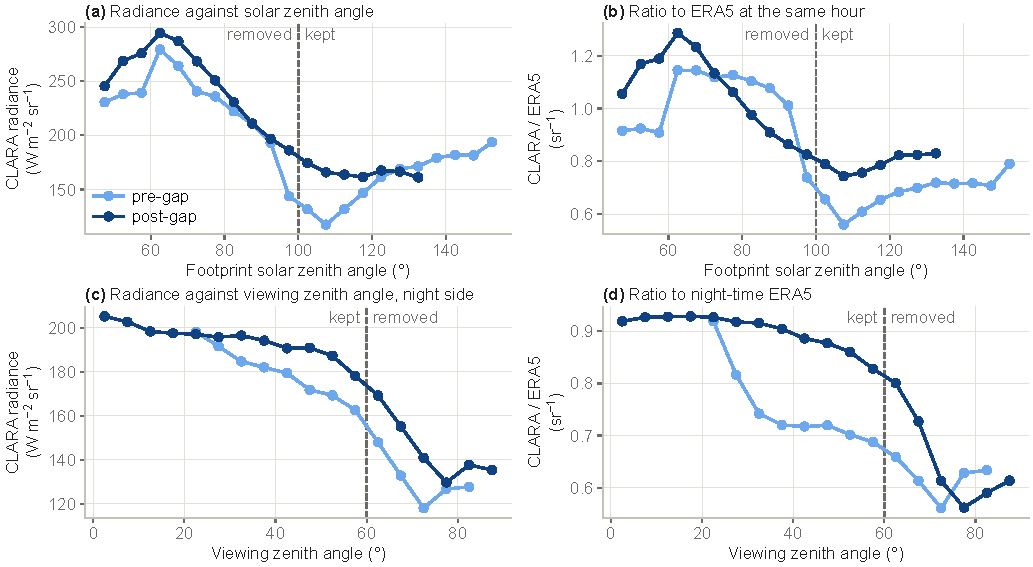
\includegraphics{physics}
\caption{\textbf{Sunlit footprints read high and steeply viewed ones low, so only night-side footprints at moderate viewing angles are kept.} Mean CLARA radiance (a, c; \Wmsr) and its ratio to ERA5 (b, d; sr$^{-1}$) in \physicsBinDeg° bins of footprint solar zenith angle (a, b; ERA5 at the same UTC hour) and of viewing zenith angle on the night side (c, d; night-time ERA5), before (light blue) and after (dark blue) the \gapSpan{} gap. Bins with fewer than \physicsMinSamples{} samples are left out; dashed lines mark the QC thresholds SZA $>\szaMin^\circ$ and VZA $\le\vzaMax^\circ$. The ratio removes the geographic pattern that the raw radiance carries. Relative to ERA5, daylit footprints read \daylitExcessMin--\daylitExcessMax\,\% high and the ratio falls steeply beyond \vzaMax°; within the kept range it still varies by up to \vzaSpreadPre\,\%, which the model treats as noise.}
\label{fig:physics}
\end{figure*}

\begin{figure}[t]
\centering
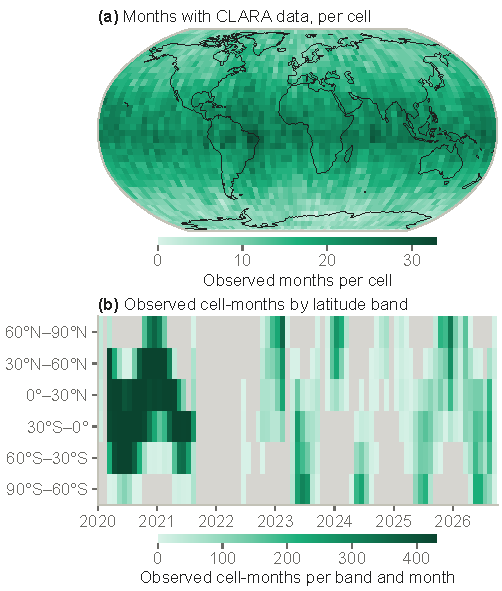
\includegraphics{data_coverage}
\caption{\textbf{CLARA's coverage is patchy in space and much sparser after the gap than before it.} (a) Months, of the \monthsObserved{} with data, in which each \gridRes° cell holds at least one quality-checked sample; (b) observed cell-months per latitude band and month. Grey: no observation, including the \gapStart{} -- \gapEnd{} gap. A month with data covers a median of \areaObsMedPre\,\% of the globe before the gap but \areaObsMedPost\,\% after it (at most \areaObsMaxPost\,\%), and after the gap \singleOverpassPost\,\% of the cell-months rest on a single overpass: no month is complete, so every monthly map has to be gap-filled.}
\label{fig:coverage_data}
\end{figure}

% =============================================================================
\section{How CLARA compares with ERA5 and CERES}\label{sec:eda}

\begin{itemize}
\item \plan{\textbf{ERA5 and CERES agree} on the same cell-months: bias \eraCeresBias\,\Wm, $r=\eraCeresR$, RMSE \flux{\eraCeresRmse}. The CLARA--ERA5 discrepancies therefore belong to CLARA. Consistent with \cite{loeb2022trends}.}
\item \plan{\textbf{CLARA vs ERA5 night}, \gridRes° cell-months: pooled $r=\rClaraEra$; ratio of means \ratioAll\,sr$^{-1}$; relative slope \relSlope{} (a 1\,\% change in ERA5 goes with a \relSlope\,\% change in CLARA). Night-time ERA5 is only marginally closer than 24 h ERA5 ($r$ \rClaraEraNight{} vs \rClaraEraDay).}
\item \plan{\textbf{A \stepRatio\,\% calibration step.} CLARA/ERA5 is \ratioPre\,sr$^{-1}$ before the \gapStart{} gap and \ratioPost\,sr$^{-1}$ after; at the same viewing angles (VZA \vzaMidLo--\vzaMidHi°) it is \ratioVzaMidPre{} vs \ratioVzaMidPost\,sr$^{-1}$, so it is calibration, not geometry (\cref{fig:global_eda}c). Within each period CLARA follows ERA5's month-to-month variation.}
\item \plan{\textbf{Damped spatial contrast.} Zonal-mean shape right ($r=\zonalR$), but the equator-to-pole contrast is only \zonalContrast\,\% of ERA5's (\cref{fig:zonal}).}
\item \plan{\textbf{Scales.} Residual correlogram $\corrC\,e^{-d/\corrRangeKm\,\mathrm{km}}$ (\cref{fig:correlogram}); the nugget (sampling noise) takes \nuggetShare\,\% of the residual variance; lag-1-month autocorrelation at a fixed cell only \acfLagOne. These numbers set the CV blocks and buffers (\cref{sec:cv}).}
\end{itemize}

\begin{figure}[t]
\centering
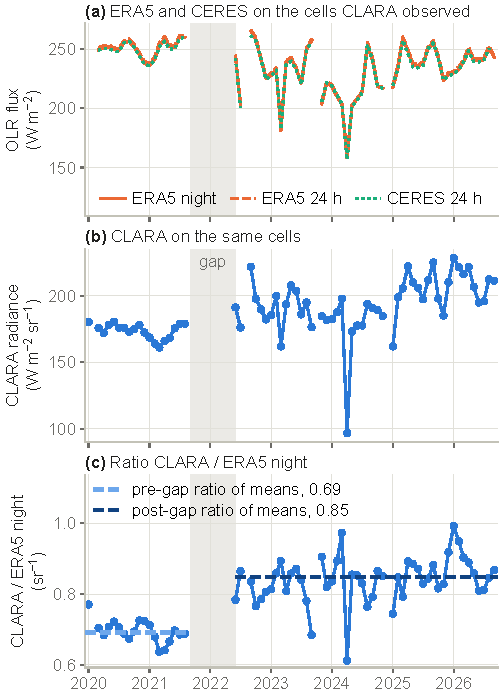
\includegraphics{global_eda}
\caption{\textbf{ERA5 and CERES agree, while CLARA's level relative to ERA5 jumps across the gap.} Monthly area-weighted means over the cells CLARA observed in each month: (a) ERA5 night-time and 24\,h and CERES 24\,h flux (\Wm); (b) CLARA radiance (\Wmsr); (c) the ratio CLARA/ERA5 night (sr$^{-1}$), with the ratio of the period means before (\ratioPre) and after (\ratioPost) the gap, dashed. Grey: the \gapStart{} -- \gapEnd{} gap; other breaks are months without data. The \stepRatio\,\% step is a change in CLARA's calibration, not in Earth's OLR, so the model carries a post-gap offset $\beta_2$.}
\label{fig:global_eda}
\end{figure}

\begin{figure}[t]
\centering
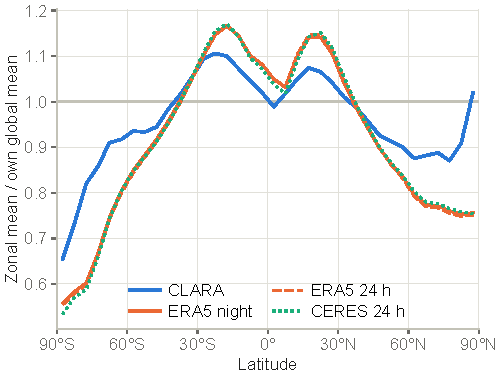
\includegraphics{zonal}
\caption{\textbf{CLARA has the right zonal shape but a damped equator-to-pole contrast.} Zonal means over the observed cell-months of CLARA, ERA5 night, ERA5 24\,h and CERES 24\,h, each divided by its own area-weighted global mean so that radiance and flux share one unitless axis. CLARA's profile correlates with ERA5 night at $r=\zonalR$, but its contrast is only \zonalContrast\,\% of ERA5's; the model absorbs this in the ERA5 slope $\beta_1$ (relative value \betaOneRel).}
\label{fig:zonal}
\end{figure}

\begin{figure}[t]
\centering
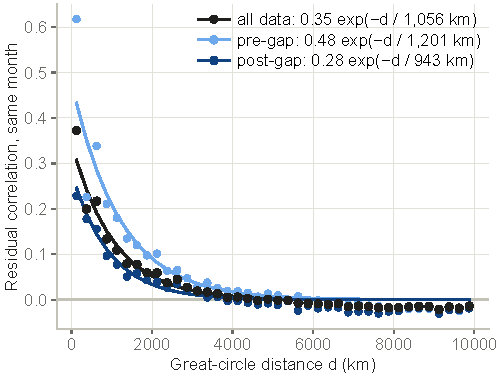
\includegraphics{correlogram}
\caption{\textbf{The CLARA--ERA5 residual is correlated over about a thousand kilometres, but most of its variance is sampling noise.} Correlation of pairs of residuals in the same month (CLARA minus a linear fit on ERA5 night, monthly means removed) against great-circle distance $d$, with weighted fits $c\,e^{-d/L}$ for all data and for each period (legend). For all data $c=\corrC$ and $L=\corrRangeKm$\,km, so the nugget $1-c$ takes \nuggetShare\,\% of the residual variance. These scales set the \SI{\cvBufferKm}{km} buffers of the spatial CV blocks (\cref{sec:cv}).}
\label{fig:correlogram}
\end{figure}

% =============================================================================
\section{Statistical model}\label{sec:model}

\subsection{Mean function and Gaussian process}
The unit of analysis is a \gridRes° cell in one calendar month. CLARA observed \nObs{} such cell-months; the prediction grid covers all \nCells{} cells in each of the \nMonthsGrid{} months from \firstMonth{} to \lastMonth, \nGrid{} cell-months in total. For cell-month $i$ we model the CLARA mean radiance $y_i$ as
\begin{equation}
y_i = \beta_0 + \beta_1 e_i + \beta_2 s_i + f(\mathbf{x}_i) + \varepsilon_i,\quad
\varepsilon_i \sim \mathcal{N}\!\Big(0,\ \sigma_0^2 + \tfrac{\sigma_1^2}{n_i}\Big)
\label{eq:model}
\end{equation}
where $e_i$ is the night-time ERA5 OLR of the cell (\Wm), $s_i=\mathbf{1}[t_i\ge\text{\gapStart}]$ marks the months from the start of the gap onwards, and $n_i$ is the number of overpasses behind $y_i$. The intercept $\beta_0$ and the step $\beta_2$ are in \Wmsr; the slope $\beta_1$, in sr$^{-1}$, converts ERA5's flux into CLARA's radiance, so the two are never subtracted. The step absorbs the calibration change across the gap (\cref{sec:eda}); the gap months, which have no data, are assigned to the post-gap level. The noise variance has a floor $\sigma_0^2$ and a part $\sigma_1^2/n_i$ that shrinks with the number of overpasses, because samples within one overpass are strongly correlated (\cref{sec:qc}). The regression coefficients $\bm\beta=(\beta_0,\beta_1,\beta_2)$ and the covariance parameters $\theta$ are estimated together, as in generalised least squares, rather than fitting the regression first and the GP to its residuals.
\begin{gather}
k(\mathbf{x},\mathbf{x}') = \sigma_A^2\,\kappa(r_A) + \sigma_B^2\,\kappa(r_B), \label{eq:kernel}\\
r_A^2 = \tfrac{\lVert\mathbf{u}-\mathbf{u}'\rVert^2}{\ell_{sA}^2} + \tfrac{\lVert\mathbf{c}-\mathbf{c}'\rVert^2}{\ell_{\mathrm{season}}^2},\quad
r_B^2 = \tfrac{\lVert\mathbf{u}-\mathbf{u}'\rVert^2}{\ell_{sB}^2} + \tfrac{(t-t')^2}{\ell_t^2} \notag
\end{gather}
The latent field $f$ is a zero-mean GP whose covariance (\cref{eq:kernel}) is the sum of two components with variances $\sigma_A^2$ and $\sigma_B^2$. A cell centre is represented by its unit vector $\mathbf{u}\in\mathbb{R}^3$ and distances are chords, so the poles and the dateline need no special treatment and every correlation function below stays positive definite on the sphere. Component A pairs space with the seasonal cycle, $\mathbf{c}$ being the month's position on a unit circle so that December lies next to January; it describes a discrepancy pattern that recurs every year. Component B pairs space with time $t$, in years since \timeOrigin, and describes drift that does not recur. Each component has its own length scales $\ell$, and $\theta=(\sigma_A,\ell_{sA},\ell_{\mathrm{season}},\sigma_B,\ell_{sB},\ell_t,\sigma_0,\sigma_1)$. We compare three correlation functions $\kappa$ that differ only in how smooth the field is: the exponential $e^{-r}$, the Gaussian $e^{-r^2/2}$ and the Mat\'ern-3/2 $(1+\sqrt3\,r)\,e^{-\sqrt3\,r}$ \cite{rasmussen2006gpml}.

\subsection{Inference and prediction}
An exact GP on \nObs{} observations is costly, so we maximise the collapsed variational lower bound of \citet{titsias2009vfe} on the log marginal likelihood, extended to the observation-specific noise of \cref{eq:model}, with $M=\nInducing$ inducing inputs placed by k-means. The bound is maximised with L-BFGS from \nStarts{} fixed starting points, and $\hat{\bm\beta}$ and $\hat\theta$ are plugged in; their uncertainty is not propagated. A unit test checks that the bound equals the exact log marginal likelihood when the inducing inputs are the training inputs. For every cell-month of the grid we report the posterior mean and the latent posterior SD, the uncertainty of the monthly mean itself. To score a held-out cell-month from $n_*$ overpasses we add its observation noise, $\sigma_0^2+\sigma_1^2/n_*$, to the latent variance. For month $t$, with $A_i$ the area of cell $i$ (all \nCells{} cells, polar-day cells included) and $\hat\mu_{i,t}$ its posterior mean,
\begin{equation}
\begin{gathered}
G_t=\sum_i w_i\,\hat\mu_{i,t},\qquad w_i=\frac{A_i}{\sum_j A_j},\\
\operatorname{Var}(G_t\mid\mathbf{y})=\mathbf{w}^\top\mathbf{C}_t\,\mathbf{w},
\end{gathered}
\label{eq:globalmean}
\end{equation}
where $\mathbf{C}_t$ is the posterior covariance of the month's latent values. Neighbouring cells share their errors, so the off-diagonal of $\mathbf{C}_t$ matters: treating the cells as independent would make the SD of $G_t$ \sdRatioMin--\sdRatioMax{} times too small (median \sdRatioMedian).

\subsection{Validation design}\label{sec:cv}
Neighbouring cells and months are correlated, so randomly held-out cell-months would have close neighbours in the training data. We therefore use blocked cross-validation \cite{roberts2017blockcv} with three designs. The \nFoldsSpatial{} spatial folds each hold out a \cvBlockDeg°$\times$\cvBlockDeg° block and drop training cells within \cvBufferKm\,km of it, the fitted correlation range rounded up (\cref{fig:correlogram}). The \nFoldsTemporal{} temporal folds each hold out a \cvWindowMonths-month window, with a buffer of \cvBufferMonths{} month on either side. The \nFoldsJoint{} joint folds hold out a block during a window, with both buffers. The \nFolds{} folds are fixed and checksummed, so every model sees identical splits, and everything learned from data (the ERA5 smoothing radius, the standardisation, the inducing inputs, $\bm\beta$ and $\theta$) is learned within each fold from its training rows only. We score the RMSE (\Wmsr), the CRPS \cite{gneiting2007scoring}, the negative log predictive density, the coverage of central predictive intervals and the PIT histogram. The rule for choosing the kernel was fixed before any fit: the lowest mean, over the three designs, of the mean fold RMSE. Three reduced models are scored on the same folds: the GP without ERA5, the regression on ERA5 without the GP, and a constant per period.

% =============================================================================
\section{Results}\label{sec:results}

\subsection{Kernel selection}
The exponential kernel has the lowest primary score, \clara{\scoreExp}, against \scoreGauss{} for the Gaussian and \scoreMatern{} for the Mat\'ern-3/2 kernel (\cref{tab:kernels}), and is used for all maps. The margin is small: in every design, the paired fold-bootstrap \ciLevel\,\% interval of the RMSE difference between the exponential kernel and each alternative contains zero. The rule fixed in advance therefore picks a kernel for the maps; it does not show that the exponential kernel is better. The sparse approximation does not decide the ranking either: changing the number of inducing inputs from \mSensLo{} to \mSensHi{} moves the exponential kernel's RMSE by at most \clara{\mSensMax} and never reorders the kernels.

\begin{table}[t]
\centering\small
\caption{Mean fold RMSE (\Wmsr) by kernel and CV type. Lower is better; the score is the mean of the three columns.}
\label{tab:kernels}
\begin{tabular}{@{}lcccc@{}}
\toprule
Kernel & Spatial & Temporal & Joint & Score \\
\midrule
\tabKernelRows
\bottomrule
\end{tabular}
\end{table}

\subsection{What ERA5 and the GP each add}
Both ingredients pay off, and either alone already recovers most of the gain (\cref{tab:ablation,fig:ablation}). Against a constant per period (\clara{\scoreConst}), the GP without ERA5 lowers the primary score to \scoreGPonly{} ($\pctGPonly\,\%$), the regression on ERA5 without the GP to \scoreERAonly{} ($\pctERAonly\,\%$), and the two together to \scoreExp{} ($\pctBoth\,\%$). Paired on the same folds, removing ERA5 from the GP raises the RMSE by \clara{\dEraSpatial} for held-out regions, \dEraTemporal{} for held-out half-years and \dEraJoint{} for both. Removing the GP from the ERA5 regression raises it by \dGpSpatial{} for held-out regions and \dGpJoint{} for both, and changes it by $\dGpTemporal$, not significantly, for held-out half-years. ERA5 helps most where whole regions are missing, the GP where regions and months are missing together; for a missing half-year neither adds much once the other is in the model.

\begin{table}[t]
\centering\small
\caption{$2\times2$ ablation on the same \nFolds{} folds: primary score (\Wmsr) and change relative to the per-period constant.}
\label{tab:ablation}
\begin{tabular}{@{}lcc@{}}
\toprule
 & with ERA5 & without ERA5 \\
\midrule
\tabAblationRows
\bottomrule
\end{tabular}
\end{table}

\begin{figure*}[t]
\centering
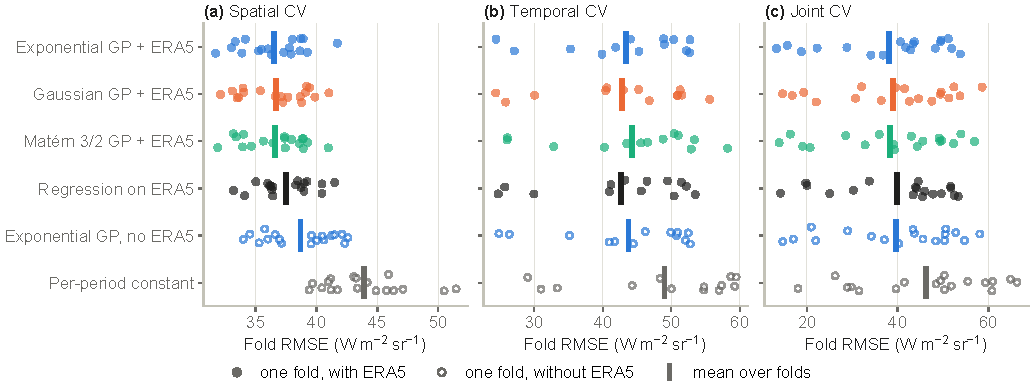
\includegraphics{model_comparison}
\caption{\textbf{ERA5 and the GP each lower the error, and the three kernels cannot be told apart.} RMSE (\Wmsr) of every held-out fold for the three GP kernels with ERA5 and the three reduced models of the $2\times2$ ablation, on identical folds: (a) \nFoldsSpatial{} spatial, (b) \nFoldsTemporal{} temporal, (c) \nFoldsJoint{} joint. Dots: single folds (hollow: without ERA5), spread vertically for legibility; bars: mean over folds; rows ordered by the primary score. The folds differ far more than the models, so models are compared through paired differences on the same folds (\cref{tab:ablation}); from the per-period constant to the exponential GP with ERA5 the score drops from \clara{\scoreConst} to \clara{\scoreExp} (\pctBoth\,\%).}
\label{fig:ablation}
\end{figure*}

\subsection{Fitted parameters}
At the means, a 1\,\% change in ERA5 changes the prediction by \betaOneRel\,\% (\cref{tab:params}): CLARA's spatial contrasts are damped, as in the exploratory analysis (\cref{sec:eda}). The step $\beta_2=\clara{\betaTwo}$ is the calibration change across the gap. The noise is almost entirely per overpass, with $\sigma_0$ close to zero, and accounts for \noiseShareVarY\,\% of the variance of the observed cell-month means. All chordal length scales exceed \maxChord, the largest chord on the unit sphere, and the time scale is $\ell_t=\tLength$ years: the latent field is close to a global offset plus a slow drift. The fine structure of the maps therefore comes from ERA5, through $\beta_1$, not from the GP.

\begin{table}[t]
\centering\small
\caption{Full-data fit, exponential kernel.}
\label{tab:params}
\begin{tabular}{@{}lr@{}}
\toprule
Parameter & Value \\
\midrule
\tabParamRows
\bottomrule
\end{tabular}
\end{table}

\subsection{Where the model errs, and calibration}
Errors are about twice as large after the gap as before it: \rmsePostLo--\clara{\rmsePostHi} against \rmsePreLo--\rmsePreHi{} across the three designs (\cref{tab:rmse_band}). Split by period, \bandWorstPre{} is the worst band before the gap (\clara{\rmseWorstPre}, spatial CV) but the best after it (\clara{\rmseWorstPost}): \postShareWorst\,\% of its held-out cell-months are post-gap. After the gap \singleMinPost--\singleMaxPost\,\% of the held-out cell-months rest on a single overpass, and the observation noise (SD \noiseSdMinPost--\clara{\noiseSdMaxPost}) accounts for \noiseMseMinPost--\noiseMseMaxPost\,\% of the mean squared error in every band. Most of the post-gap error is sampling noise that no model of the mean can remove.\par The \coverNominalHigh\,\% predictive intervals cover \coverMin--\coverMax\,\% of the held-out cell-months (\cref{fig:coverage}). Observation noise dominates the predictive variance, so this mainly tests the noise model. The latent part is tested by whole held-out half-years, and there it is too narrow: the \coverNominalHalf\,\% interval covers a fraction of only \coverHalfTemporal, and the PIT histogram peaks at its edges (\cref{fig:pit}). Far in time from the nearest observations, the uncertainty maps are therefore a lower bound.

\begin{table}[t]
\centering\small
\caption{RMSE (\Wmsr) of the exponential GP by latitude band, before (pre) and after (post) the \gapStart{} -- \gapEnd{} gap, pooled over the held-out cell-months of each CV type. Joint-CV cells hold \nCellJointMin--\nCellJointMax{} cell-months, the others \nCellMin--\nCellMax.}
\label{tab:rmse_band}
\setlength{\tabcolsep}{4pt}
\begin{tabular}{@{}lrrrrrr@{}}
\toprule
 & \multicolumn{2}{c}{Spatial} & \multicolumn{2}{c}{Temporal} & \multicolumn{2}{c}{Joint} \\
\cmidrule(lr){2-3}\cmidrule(lr){4-5}\cmidrule(lr){6-7}
Band & pre & post & pre & post & pre & post \\
\midrule
\tabRmseBandRows
\bottomrule
\end{tabular}
\end{table}

\begin{figure}[t]
\centering
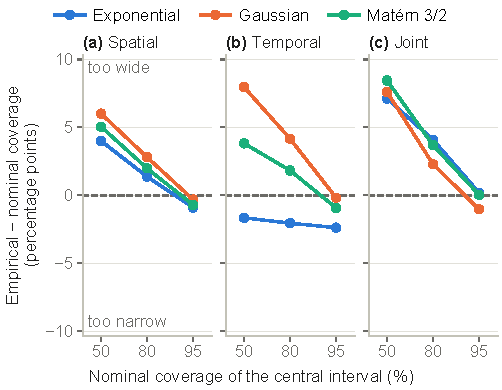
\includegraphics{coverage}
\caption{\textbf{The \coverNominalHigh\,\% predictive intervals keep close to their nominal coverage; the inner intervals are mostly too wide.} Empirical minus nominal coverage, in percentage points, of central predictive intervals for a new cell-month mean (latent variance plus observation noise) at nominal levels of \coverNominalHalf, \coverNominalMid{} and \coverNominalHigh\,\%, pooled over the held-out cell-months of each CV type (a--c); above zero the intervals are too wide. The \coverNominalHigh\,\% intervals of the exponential kernel cover \coverMin--\coverMax\,\%. Observation noise dominates the predictive variance, so coverage mainly tests the noise model; whole held-out half-years are the case where the exponential kernel's intervals are slightly too narrow (PIT in \cref{fig:pit}).}
\label{fig:coverage}
\end{figure}

\subsection{Gap-filled maps}
\Cref{fig:maps} follows one month from data to map. In \exampleMonthName{} CLARA observed \exampleCells{} cells, \exampleCoverage\,\% of the globe; the model fills the rest with ERA5's pattern, rescaled by the regression and shifted by the large-scale GP. The latent SD varies little across the globe, because the fitted length scales are global. In \gapStartName, the first month without any CLARA data, the map rests on ERA5, through the regression, and on what the GP learned from the other years: an educated estimate, not a measurement. Averaged over the globe with the full posterior covariance, the monthly mean is far better constrained than any single cell (\cref{fig:gp_global}).\par The global means of the three kernels (\cref{fig:kernel_gap}) agree before the gap (spread \clara{\kernelSpreadPre} on average) and split by \clara{\kernelSpreadMax} in its first month, \kernelSpreadMonth. After the gap they still differ by \clara{\kernelSpreadPost} on average, more than \nSD\,SD of the exponential global mean in \kernelAboveTwoSDPost{} of \nMonthsPost{} months. The choice of kernel, which cross-validation cannot settle, is therefore a source of uncertainty that the stated SD does not include, and it matters most where the data are fewest.

\begin{figure*}[t]
\centering
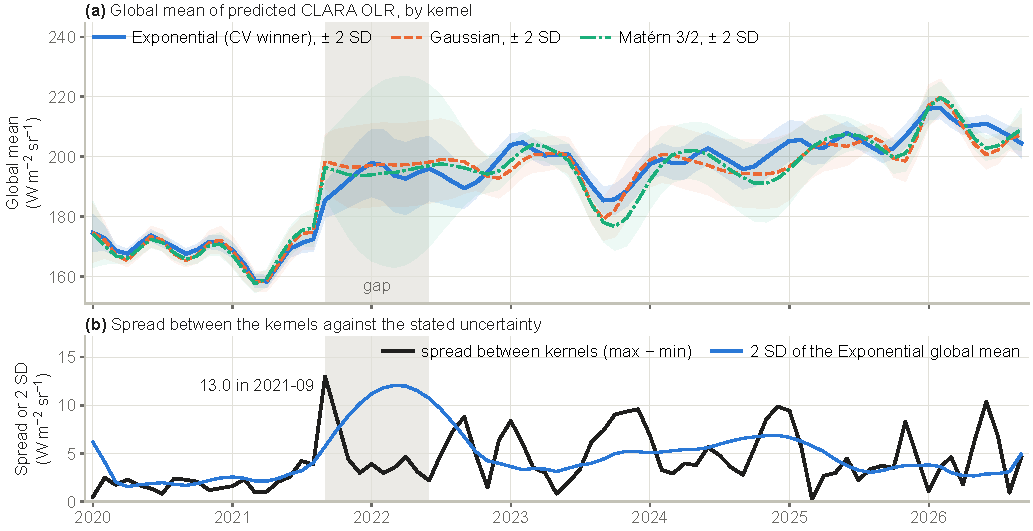
\includegraphics{kernel_gap}
\caption{\textbf{The three kernels, indistinguishable in cross-validation, disagree most where there are no data: in the gap.} (a) Monthly global mean $G_t$ (\cref{eq:globalmean}) of predicted CLARA OLR (\Wmsr) from each kernel's full-data fit, with $\pm\nSD$\,SD from its full posterior covariance; grey: no CLARA data (\gapStart{} -- \gapEnd). (b) Spread between the kernels (max $-$ min) against \nSD\,SD of the exponential global mean. The kernels agree before the gap (mean spread \clara{\kernelSpreadPre}), split by \clara{\kernelSpreadMax} in \kernelSpreadMonth, and after it still differ by more than \nSD\,SD in \kernelAboveTwoSDPost{} of \nMonthsPost{} months: the choice of kernel is a source of uncertainty that the stated SD does not include.}
\label{fig:kernel_gap}
\end{figure*}

\begin{figure*}[t]
\centering
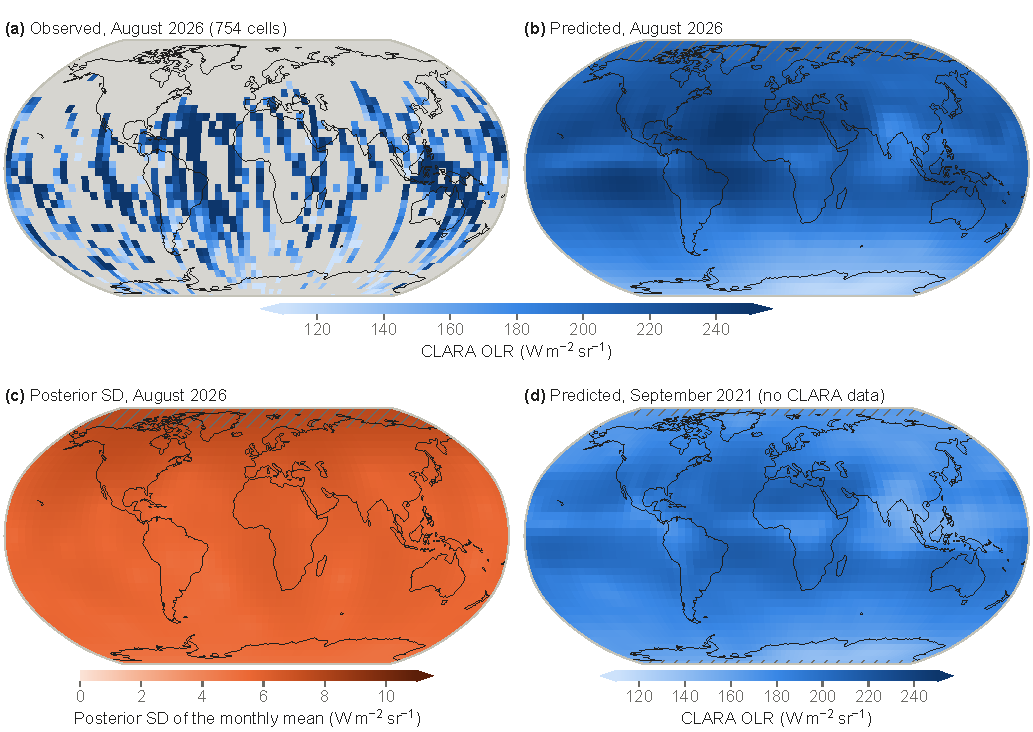
\includegraphics{maps}
\caption{\textbf{From patchy measurements to a complete map with an uncertainty for every cell.} (a) Observed CLARA cell-month means in \exampleMonthName{} (\exampleCells{} cells, \exampleCoverage\,\% of the globe; grey: not observed); (b) the exponential GP's prediction for the same month; (c) its posterior SD of the monthly mean (latent, without observation noise); (d) the prediction for \gapStartName, the first month of the gap, without any CLARA data. All CLARA OLR maps of the paper share one colour scale (\Wmsr); hatched: polar day, where ERA5 has no night and the prediction is an extrapolation. The fine structure of the predicted maps is ERA5's, scaled by $\beta_1$; the SD in (c) varies little across the globe because the fitted length scales are global (\cref{tab:params}).}
\label{fig:maps}
\end{figure*}

\begin{figure}[t]
\centering
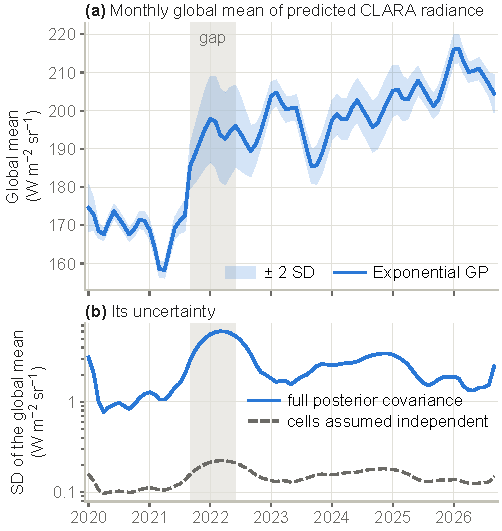
\includegraphics{global_mean}
\caption{\textbf{The monthly global mean is known to within a few \Wmsr{} outside the gap, and only the full posterior covariance gives that uncertainty honestly.} (a) Area-weighted global mean $G_t$ (\cref{eq:globalmean}) of predicted CLARA OLR (exponential GP, \Wmsr) with $\pm\nSD$\,SD from the full posterior covariance; grey: the gap. (b) The SD of $G_t$ (log scale) from the full posterior covariance and as it would be if the cells were independent. Neighbouring cells share their errors, so the full-covariance SD is \sdRatioMin--\sdRatioMax{} times the independent-cell value (median \sdRatioMedian).}
\label{fig:gp_global}
\end{figure}

% =============================================================================
\section{Software: clara-olr-gapfill}\label{sec:software}
\plan{One paragraph + one small table of commands. The tool packages the selected model: \texttt{prepare} $\to$ \texttt{fit} $\to$ \texttt{predict} $\to$ \texttt{maps} (and optional \texttt{validate}), one TOML config, any grid that divides \gridDivisor°, stage manifests so only changed stages rerun, portable model files (no pickle), synthetic demo. Reproducibility: at \gridRes° the training table and grid are identical to the research pipeline; predictions of the imported reference model agree to \toolDecimals{} decimals; a refit reaches the reference bound to $\toolBoundGap$ per observation and its maps differ by \clara{\toolMapRms} RMS. Runtime: fit $\approx$ \toolFitWallLo--\toolFitWallHi{} min on a \toolFitCores-core laptop (\toolFitCpuMin{} min of CPU time). No data distributed; CLARA from PMOD/WRC, ERA5 from CDS.} \plan{Package \texttt{clara-olr-gapfill} (CLI \texttt{clara-gapfill}); source at \url{https://github.com/camillandreozzi/OLR-gapfill-tool} \cite{andreozzi2026tool}.}

% =============================================================================
\section{Discussion}\label{sec:discussion}
\begin{itemize}
\item \plan{\textbf{What CLARA adds beyond ERA5.} Modest out-of-sample gains; most fine structure is ERA5's scaled by $\beta_1$. CLARA's own contribution is a large-scale, slowly varying offset and drift -- exactly what an absolute radiometer can say about a reanalysis.}
\item \plan{\textbf{The gap -- and after it.} One global step at the start of the gap; its timing is unknown. The kernels diverge by up to \clara{\kernelSpreadMax} in \kernelSpreadMonth, but also by \clara{\kernelSpreadPost} on average after the gap (more than \nSD\,SD in \kernelAboveTwoSDPost{} of \nMonthsPost{} months), so kernel choice is a source of uncertainty the latent SD does not include. The answer in the gap depends on assumptions (homogeneity, linear ERA5 link, smoothness).}
\item \plan{\textbf{Limitation: the \lastYear{} radiance cut} (decided: keep, do not refit). \lastYear{} inherits the \olrMinRaisedSecondYear{} lower bound (\clara{\olrMinRaisedSecond}) although its histogram trough is at \clara{\troughLastYear}, so cold-scene samples between the two are dropped and \lastYear{} cell-means in cold regions may be slightly high.} \TODO{macro for the number of \lastYear{} samples between \troughLastYear{} and \olrMinRaisedSecond{} (ask Claude Code).}
\item \plan{\textbf{Geometry and footprint.} No angular model, residual VZA effect as noise, damped contrasts; collocation with CERES footprints \cite{pmod_clara_ceres_pipeline} is the natural next step.}
\item \plan{\textbf{Diurnal sampling.} Night-only at drifting local time; ERA5 night matches it only partially; cf.\ CERES temporal interpolation \cite{doelling2013geo}.}
\item \plan{\textbf{Uncertainty.} Close to nominal in space; too narrow for whole held-out half-years; plug-in hyperparameters; VFE bound not fully converged in $M$ although predictions are stable.}
\item \plan{\textbf{Baselines not run.} DINEOF \cite{beckers2003dineof}, simple interpolation \cite{liebmann1996olr}.}
\end{itemize}

% =============================================================================
\section{Conclusions and outlook}\label{sec:conclusion}
\plan{What we showed: complete monthly maps \firstYear--\lastYear{} (\nGrid{} values with uncertainties), tested on data the model never saw. What it could enable: small, low-cost instruments from Davos complementing large missions; the same approach for other small satellites; high-accuracy radiometers giving an independent view on the absolute value of reanalysis data or uncalibrated satellite data. Outlook: angular correction, CERES footprint collocation, DINEOF on the same folds, extension as new CLARA months arrive.}

\section*{Code and data availability}
\plan{Research pipeline, folds (with checksum), tables and figures: \cite{andreozzi2026repo}. Gap-filling tool: \cite{andreozzi2026tool}. CLARA data from PMOD/WRC (\url{https://projects.pmodwrc.ch/clara/}); ERA5 from the Copernicus Climate Data Store; CERES EBAF from NASA.}

\section*{Acknowledgements}
This work was carried out at PMOD/WRC in Davos with support from Academia Raetica and from ETH Z\"urich through the ETH Studios. We thank the CLARA instrument team at PMOD/WRC for the data and for their help with them. The Gaussian-process fits were run on the Euler cluster of ETH Z\"urich. ERA5 data were provided by the Copernicus Climate Change Service, and CERES EBAF data by the NASA Langley Research Center.

\bibliographystyle{abbrvnat}
\bibliography{refs}

% =============================================================================
\clearpage
\onecolumn
\appendix
\section{Supplementary figures}

\begin{figure}[h]
\centering
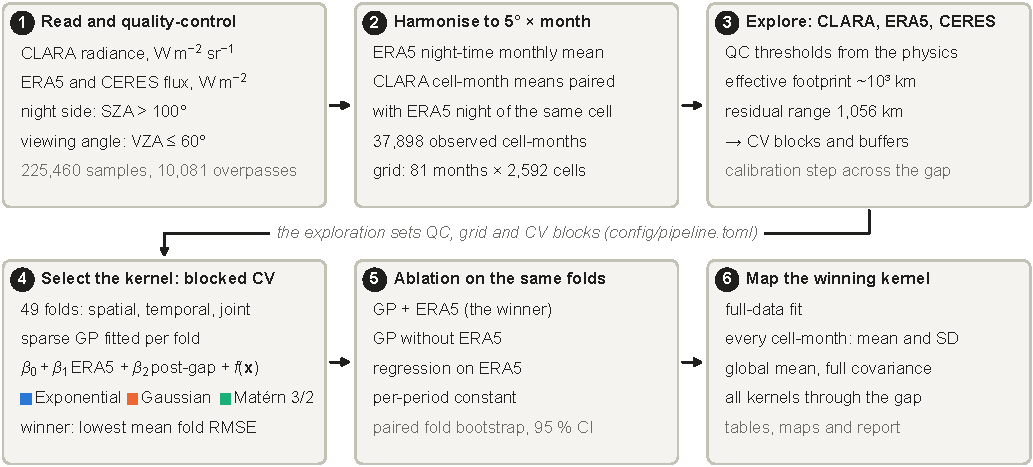
\includegraphics{pipeline}
\caption{\textbf{Every step from raw samples to maps is scripted, and the exploration sets the configuration that all later steps read.} The pipeline in six stages: (1) read and quality-control the CLARA samples and the ERA5 and CERES fields; (2) harmonise them to \gridRes° cell-months; (3) compare CLARA with ERA5 and CERES, which fixes the QC thresholds, the grid and the CV blocks; (4) select the kernel by blocked cross-validation; (5) score the reduced models of the ablation on the same folds; (6) refit the winning kernel on all data and map every cell-month. Each stage reads only the tables of the stages before it, and every number in the paper is read from those tables.}
\label{fig:pipeline}
\end{figure}

\begin{figure}[h]
\centering
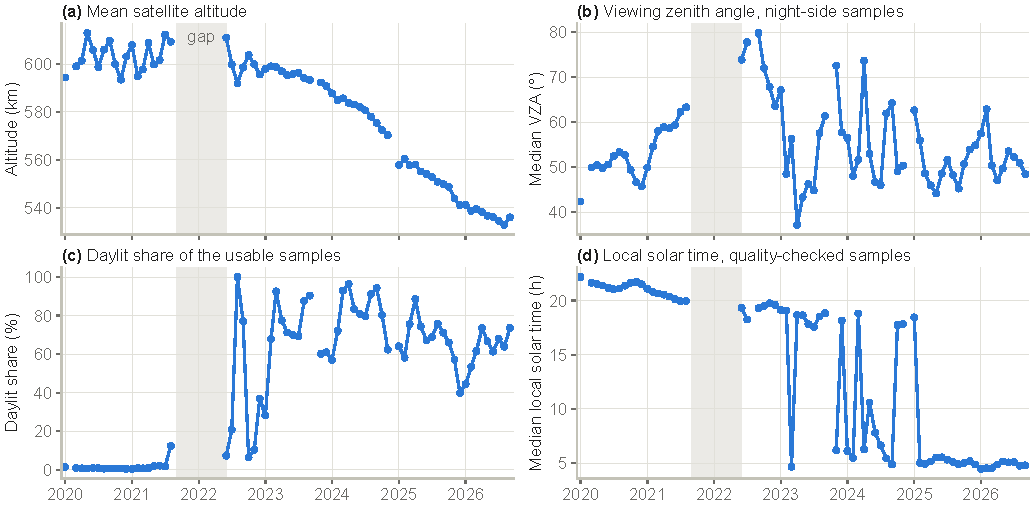
\includegraphics{geometry}
\caption{\textbf{CLARA's observing geometry drifts over the record.} Monthly (a) mean NorSat-1 altitude, (b) median viewing zenith angle of the night-side samples, (c) share of the usable samples with a daylit footprint, (d) median local solar time of the quality-checked samples; grey: the gap. The altitude falls from about \SI{\altFirst}{km} to \SI{\altLast}{km}; from \daylitFromYear{} on, \daylitShareMin--\daylitShareMax\,\% of the usable footprints of each year are daylit and are removed by the night-side cut, and the remaining samples switch between evening and morning passes. Geometry therefore changes with the period, which the post-gap offset and the noise model have to absorb.}
\label{fig:geometry}
\end{figure}

\begin{figure}[h]
\centering
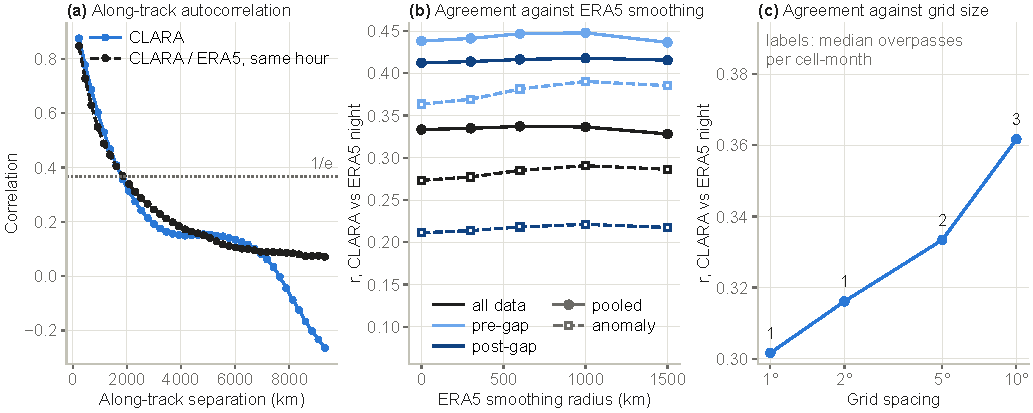
\includegraphics{resolution}
\caption{\textbf{CLARA carries structure only on scales of about $\effFootprintOrder$\,km, so a \gridRes° grid is fine enough.} (a) Correlation between quality-checked samples of the same overpass against their along-track separation, for CLARA and for its ratio to hour-matched ERA5 (first lag: $r=\rAlongTrack$; dotted: $1/e$). (b) Correlation of CLARA with ERA5 night on \gridRes° cell-months against the radius of the spherical cap that smooths ERA5: pooled, and for anomalies from each latitude band's monthly mean, for all data and each period. (c) The pooled correlation against grid spacing; labels give the median number of overpasses per cell-month. Agreement barely changes with smoothing and rises with coarser cells as more overpasses are averaged: sampling noise, not resolution, limits the agreement.}
\label{fig:resolution}
\end{figure}

\begin{figure}[h]
\centering
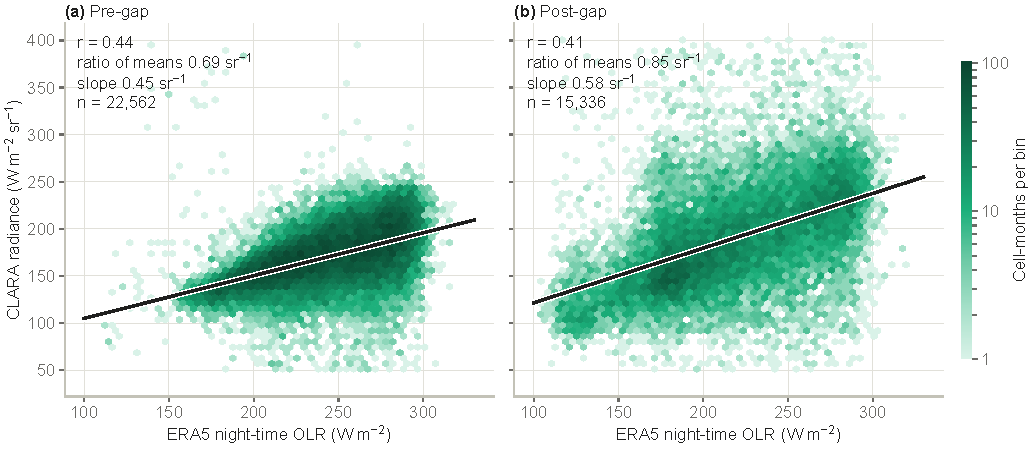
\includegraphics{joint_scatter}
\caption{\textbf{Cell by cell, CLARA follows ERA5 only loosely, at a higher level and with a steeper slope after the gap.} CLARA (\Wmsr) against ERA5 night-time OLR (\Wm) for every observed \gridRes° cell-month before (a) and after (b) the gap; shading: cell-months per hexagonal bin (log scale, one scale for both panels); black: area-weighted linear fit, with its statistics in each panel. Pooled over both periods $r=\rClaraEra$: most of the scatter is CLARA's sampling noise, which the noise term $\sigma_0^2+\sigma_1^2/n_i$ of the model absorbs.}
\label{fig:joint_scatter}
\end{figure}

\begin{figure}[h]
\centering
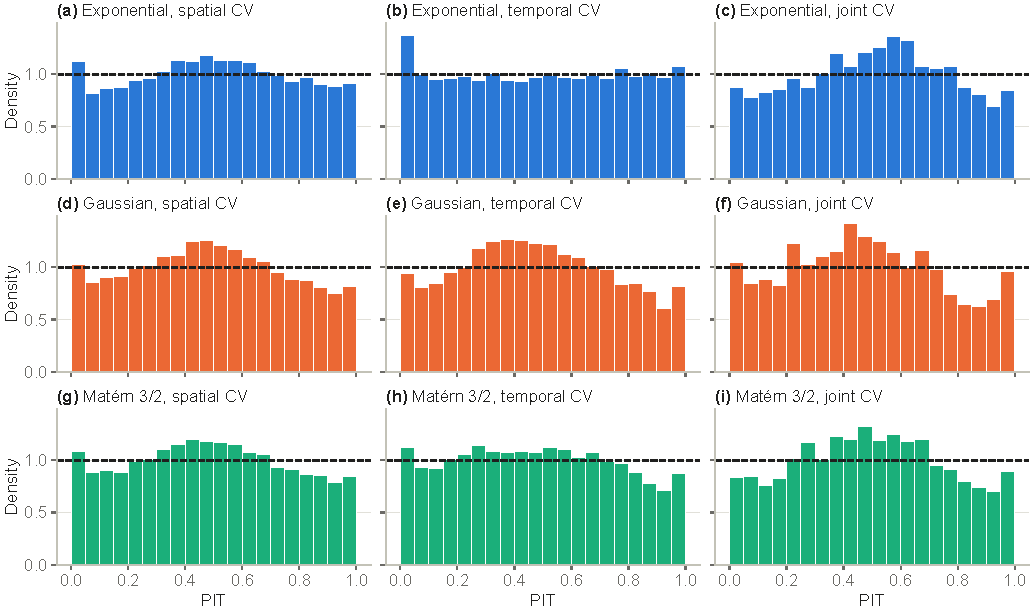
\includegraphics{pit}
\caption{\textbf{The predictive distributions are roughly calibrated, mostly a little too wide.} Histograms of the probability integral transform (PIT) of every held-out cell-month, by kernel (rows) and CV type (columns); dashed: the flat histogram of a calibrated forecast. A hump means intervals that are too wide, a U shape intervals too narrow, a slope a bias. Most panels show a mild hump; for whole held-out half-years the exponential kernel has a peak in the lowest bin (b): observations below the predicted range.}
\label{fig:pit}
\end{figure}

\begin{figure}[h]
\centering
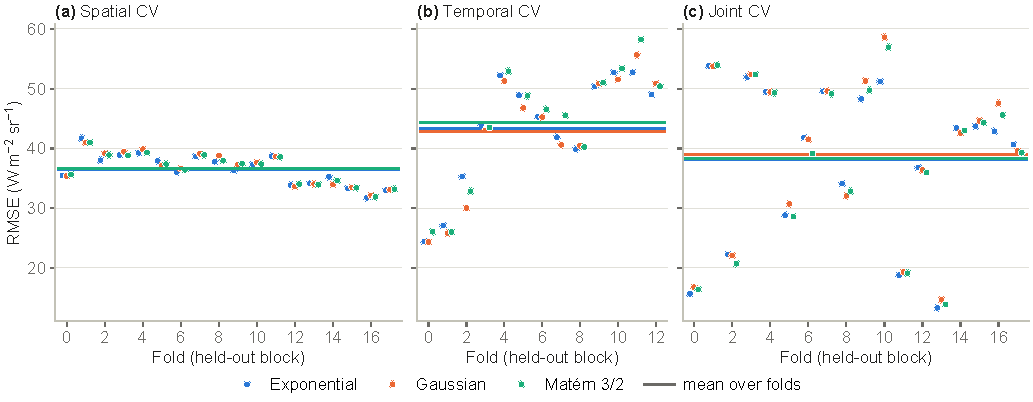
\includegraphics{rmse_by_fold}
\caption{\textbf{Which block is held out matters far more than which kernel is used.} RMSE (\Wmsr) of the three kernels on each held-out block: (a) \nFoldsSpatial{} spatial, (b) \nFoldsTemporal{} temporal and (c) \nFoldsJoint{} joint folds; lines: mean over folds. Across folds the RMSE ranges over tens of \Wmsr, while on the same fold the kernels differ by a few, so the kernels are compared through paired differences (\cref{tab:kernels}).}
\label{fig:rmse_fold}
\end{figure}

\begin{figure}[h]
\centering
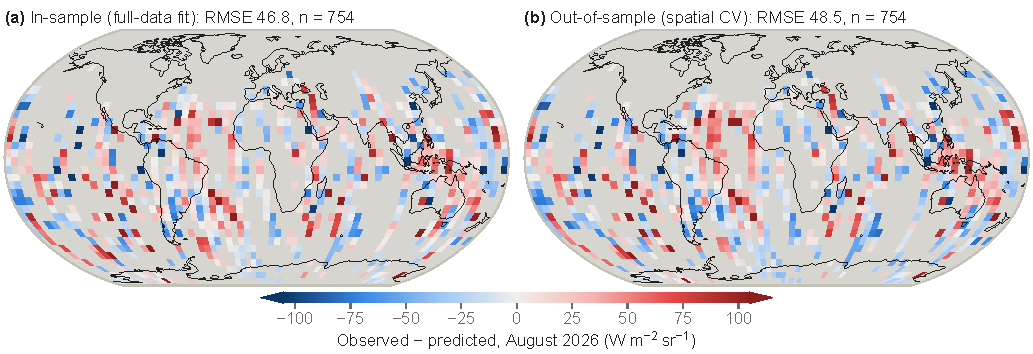
\includegraphics{residuals}
\caption{\textbf{In-sample and out-of-sample residuals are of similar size and mostly cell-to-cell noise.} Observed minus predicted CLARA OLR (\Wmsr) in \exampleMonthName: (a) in-sample, from the full-data fit; (b) out-of-sample, from the spatial CV fold that held out each cell's block. Grey: not observed; one diverging scale for both panels and all months. The error grows only a little out of sample, as expected when observation noise, not the distance to the nearest data, dominates it.}
\label{fig:residuals}
\end{figure}

\end{document}
